\documentclass[openany]{book}

\usepackage[italian]{babel}

\usepackage[a4paper,top=2cm,bottom=2cm,left=2cm,right=2cm,marginparwidth=1.75cm]{geometry}
\usepackage{needspace}
% \usepackage{showframe}
\usepackage{enumitem} % per personalizzare enumerate
\usepackage{amsmath, amssymb}
\usepackage{graphicx}
\usepackage[hidelinks]{hyperref}
\usepackage{tcolorbox}
\usepackage{tikz}
\tikzset{every picture/.style={baseline=-0.5ex}}
% Define colors for name-verb analysis and legend
% https://www.overleaf.com/learn/latex/Using_colors_in_LaTeX
\usepackage{soul}
\usepackage[dvipsnames]{xcolor}
\colorlet{ColorClass}{Cyan}
\colorlet{ColorAttr}{Green}
\colorlet{ColorFunc}{Yellow}
\colorlet{ColorActor}{Red}
\colorlet{ColorClassActor}{Thistle}
\newcommand{\Class}[1]{\sethlcolor{ColorClass}\hl{#1}}
\newcommand{\Attr}[1]{\sethlcolor{ColorAttr}\hl{#1}}
\newcommand{\Func}[1]{\sethlcolor{ColorFunc}\hl{#1}}
\newcommand{\Actor}[1]{\sethlcolor{ColorActor}\hl{#1}}
\newcommand{\ClassActor}[1]{\sethlcolor{ColorClassActor}\hl{#1}}
\usepackage[italian]{babel}
\usepackage{tabularx}
\usepackage{amsmath}

\newcommand{\Req}[2]{\textsc{#1$_{#2}$}}


\usepackage{tabularray}
\UseTblrLibrary{varwidth}
\usepackage{enumitem}
\usepackage{eurosym}
\usepackage{minted}
\usepackage{tablefootnote}

\usepackage{tikz}
\usetikzlibrary{shapes.geometric, arrows, positioning, fit}

\usepackage{hyperref}

% Tabella per gli scenari
\NewTblrEnviron{scenery}
\SetTblrInner[scenery]{
	hlines, vlines,
	% rowsep=1.5pt,
	row{1} = {bg=black, fg=white, font=\bfseries},
	column{1} = {font=\bfseries},
	measure=vbox, stretch=-1
}

% Tabella per il category partition testing
\NewTblrEnviron{partest}
\SetTblrInner[partest]{
	hlines, vlines,
	row{1} = {font=\bfseries},
	measure=vbox, stretch=-1
}

% Tabella per le test suite
\NewTblrEnviron{testsuite}
\SetTblrInner[testsuite]{
	hlines, vlines,
	row{1} = {font=\bfseries}
}

% This command includes an exported pdf table in the document, if it exists. Otherwise it includes table.tex.
% Variante senza float per evitare problemi di spazio bianco
% Improved version that handles spacing better
\newcommand{\IncludeTable}[2][!h]{
	\IfFileExists{#2.pdf}{%
		\begin{figure}[#1]%
			\centering%
			\includegraphics[width=\linewidth]{#2.pdf}%
		\end{figure}%
	}{
		\input{#2}%
	}
}

% \includeonly{chapters/implementazione}

\begin{document}

\begin{titlepage}

    \centering
    {\scshape\LARGE Università degli Studi di Federico Secondo \par}
    \vspace{1cm}
    {\scshape\Large Corso di Laurea in NomeCorso \par}
    \vfill
    {\huge\bfseries Titolo della Relazione \par}
    \vspace{2cm}
    {\Large Autore: Nome Cognome \par}
    \vspace{0.5cm}
    {\Large Matricola: 123456 \par}
    \vspace{0.5cm}
    {\Large Anno Accademico: 2024/2025 \par}
    \vfill


% Indice
\tableofcontents
\newpage
\end{titlepage}


\chapter{Specifiche Informali}
Si intende sviluppare un sistema software per la gestione della vendita di biglietti per eventi, con funzionalità di controllo accessi in fase di partecipazione. Il sistema è destinato sia agli utenti finali (partecipanti) sia agli amministratori che organizzano e gestiscono gli eventi.\\

\noindent Il sistema consente la registrazione di utenti, che devono fornire nome, cognome, indirizzo e-mail e password. Ogni utente dispone di un profilo personale, accessibile tramite autenticazione, dove può visualizzare e gestire le informazioni del proprio account, modificare i dati personali, e consultare lo storico dei biglietti acquistati ed opzionalmente la propria immagine del profilo. Ogni profilo mostra opzionalmente anche il numero totale di eventi ha cui l’utente ha partecipato.\\

\noindent Gli amministratori della piattaforma possono creare nuovi eventi, specificando per ciascuno titolo, descrizione, data, orario, luogo e numero massimo di partecipanti. Gli eventi pubblicati sono consultabili dagli utenti registrati tramite un catalogo eventi, filtrabile opzionalmente per data o località.\\

\noindent Durante il processo di acquisto, l’utente seleziona un evento e riceve un biglietto elettronico, identificato da un codice univoco. Il biglietto contiene: nome dell’evento, data, orario, nome del partecipante e codice identificativo. I biglietti possono essere scaricati o visualizzati direttamente dal profilo utente.\\

\noindent Nel giorno dell’evento, l’utente può accedere a una apposita interfaccia grafica pensata per il controllo degli accessi. In questa interfaccia gli viene presentato l’elenco di tutti gli eventi previsti per la data odierna. L’utente seleziona l’evento a cui intende partecipare e inserisce il codice del biglietto precedentemente ricevuto. Il sistema, a questo punto, effettua una serie di verifiche: controlla che il codice del biglietto esista e sia effettivamente associato all’evento selezionato, che la data indicata sul biglietto coincida con quella odierna e che il biglietto non sia già stato utilizzato. Se tutte le condizioni risultano verificate, il sistema autorizza l’accesso e marca il biglietto come “consumato”. In caso contrario, viene restituito un messaggio di errore esplicativo che impedisce l’ingresso.\\

\noindent Il sistema mantiene traccia in tempo reale delle persone presenti a ciascun evento, aggiornando dinamicamente il numero di ingressi effettuati. Gli amministratori possono accedere a un pannello di gestione per ogni evento. Per gli eventi odierni, il sistema consente di visualizzare non solo il numero di utenti registrati, ma anche l’elenco aggiornato degli utenti effettivamente presenti in quel momento. Per gli eventi passati, invece, l’amministratore potrà accedere unicamente al numero totale di partecipanti che hanno avuto accesso, senza possibilità di consultare i nomi.\\

\noindent L’applicazione deve essere accessibile via web da dispositivi desktop e mobili, offrire un’interfaccia grafica chiara e intuitiva, e implementare meccanismi di sicurezza per la protezione dei dati personali, l’autenticazione degli utenti e l’integrità dei biglietti elettronici.




\chapter{Analisi e specifica dei requisiti}
\section{Analisi nomi-verbi}


\Func{Il sistema consente la registrazione} di \Actor{utenti}, che devono fornire \Attr{nome, cognome, indirizzo e-mail e password}. Ogni cliente dispone di un profilo personale, accessibile tramite \Func{autenticazione,} dove \Func{pu\`{o} visualizzare e gestire le informazioni del proprio account, modificare i dati personali, e consultare lo storico dei biglietti acquistati ed opzionalmente la propria immagine del profilo. Ogni profilo mostra opzionalmente anche il numero totale di eventi a cui l’cliente ha partecipato}.

Gli \ClassActor{amministratori} della piattaforma possono \Func{creare nuovi eventi}, specificando per ciascuno \Attr{titolo, descrizione, data, orario, luogo e numero massimo di partecipanti}. \Func{Gli eventi pubblicati sono consultabili dagli} \ClassActor{utenti registrati} \Func{tramite un catalogo eventi, filtrabile opzionalmente per data o localit\`{a}}.

Durante il processo di \Func{acquisto}, l’cliente seleziona un evento e riceve un \Class{biglietto elettronico}, identificato da un \Attr{codice univoco}. Il biglietto contiene: \Attr{nome dell’evento, data, orario, nome del partecipante e codice identificativo}. \Func{I biglietti possono essere scaricati o visualizzati} direttamente dal profilo cliente.

Nel giorno dell’evento, l’cliente pu\`{o} accedere a una apposita interfaccia grafica pensata per il controllo degli accessi. In questa interfaccia gli viene presentato l’elenco di tutti gli eventi previsti per la data odierna. L’cliente \Func{seleziona l’evento a cui intende partecipare} e inserisce il codice del biglietto precedentemente ricevuto. \Func{Il sistema}, a questo punto, \Func{effettua una serie di verifiche}: controlla che il codice del biglietto esista e sia effettivamente associato all’evento selezionato, che la data indicata sul biglietto coincida con quella odierna e che il biglietto non sia gi\`{a} stato utilizzato. Se tutte le condizioni risultano verificate, il sistema autorizza l’accesso e marca il biglietto come “consumato”. In caso contrario, viene restituito un messaggio di errore esplicativo che impedisce l’ingresso.

\Func{Il sistema mantiene traccia in tempo reale delle persone presenti a ciascun evento, aggiornando dinamicamente il numero di ingressi effettuati}. Gli amministratori possono \Func{accedere a un pannello di gestione per ogni evento. Per gli eventi odierni, il sistema consente di visualizzare non solo il numero di utenti registrati, ma anche l’elenco aggiornato degli utenti effettivamente presenti in quel momento. Per gli eventi passati, invece, l’amministratore potr\`{a} accedere anche al numero totale di partecipanti che hanno avuto accesso}, senza possibilit\`{a} di consultarne i nomi.

L’applicazione deve essere accessibile via web da dispositivi desktop e mobili, offrire un’interfaccia grafica chiara e intuitiva, e implementare meccanismi di sicurezza per la protezione dei dati personali, l’autenticazione degli utenti e l’integrit\`{a} dei biglietti elettronici.

\bigskip
\vspace{1cm}
\noindent\textbf{\underline{LEGENDA}}\\[0.5em]
\begin{tabular}{ll}
\sethlcolor{ColorClass}\hl{\textbf{Classe}} \\
\sethlcolor{ColorAttr}\hl{\textbf{Attributo}} \\
\sethlcolor{ColorFunc}\hl{\textbf{Funzionalit\`{a}}}\\
\sethlcolor{ColorActor}\hl{\textbf{Attore}}\\
\sethlcolor{ColorClassActor}\hl{\textbf{Classe-Attore}}
\end{tabular}

\newpage
\section{Revisione dei Requisiti}

\begin{enumerate}[]
    \item Il sistema deve consentire ad un cliente di registrarsi
    \item La registrazione consiste nell’inserire nome, cognome, indirizzo e-mail e password
    \item Il sistema deve offrire una funzionalità di autenticazione
    \item il sistema deve gestire per ogni cliente lo storico dei biglietti acquistati, numero totali di eventi a cui l’cliente ha partecipato e un ImmagineProfilo
    \item Il sistema consente di visualizzare lo storico dei biglietti acquisati dall'cliente
    \item Il sistema offre una funzionalità di modifica dei dati personali
    \item Il sistema deve consentire agli amministratori la creazione di eventi
    \item Degli eventi si vuole memorizzare titolo, data, orario, luogo e numero massimo di partecipanti
    \item Il sistema deve offrire un catalogo eventi consultabile da un utente registrato
    \item Il sistema deve fornire una funzionalità di ricerca di un evento per nome, data o località.
    \item Il sistema deve consentire l’acquisto di biglietto per un evento
    \item Ogni biglietto elettronico deve avere un codice identificativo univoco
    \item il sistema deve offrirre la possibilità all'cliente di visualizzare un biglietto acquistato
    \item Il sistema deve offrire la possibilit all'cliente di scaricare un biglietto acquistato
    \item Il sistema deve consentire al cliente la partecipazione ad un evento
    \item Un biglietto marcato come consumato non può essere più essere riutilizzato
    \item Un cliente durante la fase di acquisto può comprare un solo biglietto ad esso associato
    \item Il sistema deve tener traccia dei clienti presenti a ciascun evento
    \item Il sistema deve fornire all'amministratore la possibilità di consultare informazioni aggiuntive per i suoi eventi pubblicati
    \item Il sistema deve implementare meccanismi di sicurezza per la protezione dei dati personali e per l’autenticazione degli utenti
    \item Il sistema deve offrire un’interfaccia grafica chiara e intuitiva
    \item Il sistema deve garantire l’integrità dei biglietti elettronici
    \item Il sistema deve essere accessibile da dispositivi mobili e desktop
\end{enumerate}

\section{Glossario dei termini}



\begin{tblr}{
	colspec = lXl,
	hlines, vlines,
    row{1} = {bg=gray!30, font=\bfseries}
}
\hline
	Termine & Descrizione & Sinonimi \\
\hline    
Amministratore & Amministratore della piattaforma che si occupa della gestione degli eventi & \\
Biglietto elettronico & Biglietto acquistabile e utilizzare per partecipare all'evento a cui è associato & \\
Catalogo eventi & Catalogo che contiene tutti gli eventi pubblicati dagli amministratori & \\
UtenteNonRegistrato & Una persona che intende registrarsi presso il sistema & \\
UtenteRegistrato & Un Utente che si è registrata presso il sistema & \\
Cliente & Utente registrato che acquista o partecipa a eventi. Nei diagrammi dei casi d’uso è rappresentato dall’attore "Utente"\\
\end{tblr}



\section{Classificazione dei Requisiti}

\subsection{Requisiti Funzionali}


\begin{tblr}{
	colspec = lXl,
	hlines, vlines,
	row{1} = {bg=gray!30, font=\bfseries}
}
\hline
ID & Requisito & Origine \\
\hline
\Req{rf}{01} & Il sistema offre la possibilità all’cliente di registrarsi & 1 \\
\Req{rf}{02} & Il sistema deve offrire una funzionalità di autenticazione & 3 \\
\Req{rf}{03} & il sistema deve gestire per ogni cliente lo storico dei biglietti acquistati e un ImmagineProfilo & 4 \\
\Req{rf}{04} & Il sistema consente di visualizzare lo storico dei biglietti acquistati dall'cliente & 5 \\
\Req{rf}{05} & Il sistema offre una funzionalità di modifica dei dati personali & 6 \\
\Req{rf}{06} & Il sistema deve consentire agli amministratori la creazione di eventi & 7 \\
\Req{rf}{07} & Il sistema deve offrire un catalogo eventi consultabile da un utente registrato & 9 \\
\Req{rf}{08} & Il sistema deve fornire una funzionalità di ricerca di un evento per nome, data o località. & 10 \\
\Req{rf}{09} & Il sistema deve consentire l’acquisto di biglietto per un evento & 11 \\
\Req{rf}{11} & il sistema deve offrirre la possibilit`a all’cliente di visualizzare un biglietto acquistato & 13 \\
\Req{rf}{12} & Il sistema deve offrire la possibilit all’cliente di scaricare un biglietto acquistato & 14\\
\Req{rf}{14} & Il sistema deve consentire al cliente la partecipazione ad un evento & 15 \\
\Req{rf}{15} & Il sistema deve tener traccia dei clienti presenti a ciascun evento & 18 \\
\Req{rf}{16} & Il sistema deve fornire all'amministratore la possibilità di consultare informazioni aggiuntive per i suoi eventi pubblicati & 19 \\
\end{tblr}


\subsection{Requisiti sui Dati}

\begin{tblr}{
	colspec = lXl,
	hlines, vlines,
	row{1} = {bg=gray!30, font=\bfseries}
	}
\hline
ID & Requisito & Origine \\
\hline
\Req{RD}{01} & La registrazione consiste nell’inserire nome, cognome, indirizzo e-mail e password & 2 \\
\Req{RD}{03} & Degli eventi si vuole memorizzare titolo, data, orario, luogo e numero massimo di partecipanti & 8 \\
\Req{RD}{04} & Ogni biglietto elettronico deve avere un codice identificativo univoco & 12 \\


\end{tblr}


\subsection{Vincoli/Altri Requisiti}

\begin{tblr}{
	colspec = lXl,
	hlines, vlines,
	row{1} = {bg=gray!30, font=\bfseries}
	}
    \hline
ID & Requisito & Origine \\
\hline
\Req{V}{01} & Un biglietto marcato come consumato non può essere più riutilizzato & 16 \\
\Req{V}{02} & Un cliente durante la fase di acquisto può comprare un solo biglietto ad esso associato & 17\\
\Req{V}{03} & Il sistema deve implementare meccanismi di sicurezza per la protezione dei dati personali e per l’autenti-
cazione degli utenti & 21\\
\Req{V}{04} & Il sistema deve offrire un’interfaccia grafica chiara e intuitiva & 22 \\
\Req{V}{05} & Il sistema deve garantire l’integrità dei biglietti elettronici & 23 \\
\Req{V}{06} & Il sistema deve essere accessibile da dispositivi mobili e desktop & 24 \\
    
\end{tblr}

\chapter{Modellazione dei Casi d'Uso}
\section{Attori e Casi d'Uso}
\begin{table}[!hbp]
	\centering
	\begin{tblr}{colspec=XX}
		\begin{minipage}[t]{\linewidth}
			\paragraph{Attori primari}
			\begin{itemize}[leftmargin=*]
				\item UtenteNonRegistrato
				\item UtenteRegistrato
				\item Utente
				\item Amministratore
			\end{itemize}
		\end{minipage} &
		\begin{minipage}[t]{\linewidth}
			\paragraph{Attori secondari}
			\begin{itemize}[leftmargin=*]
				\item SistemaGestioneAcquisti
			\end{itemize}
		\end{minipage} \\
	\end{tblr}
\end{table}
\begin{table}[!hbp]
	\centering
	\begin{tblr}{colspec=XX}
		\begin{minipage}[t]{\linewidth}
			\paragraph{Casi d'uso}
			\begin{enumerate}[leftmargin=*]
				\item Registrazione 
				\item Autenticazione
				\item RicercaEvento
				\item PubblicaEvento
				\item ConsultaEventiPubblicati
				\item PartecipazioneEvento
				\item AcquistoBiglietto
				\item ModificaDatiPersonali
				\item VisualizzaBiglietto
				\item ScaricaBiglietto
			\end{enumerate}
		\end{minipage} &
		\begin{minipage}[t]{\linewidth}
			\paragraph{Casi d'uso di inclusione}
			\begin{enumerate}[leftmargin=*, start=11]
                \item ConsultaCatalogoEventi
	      		\item ConsultaStoricoBiglietti
			\end{enumerate}

		\end{minipage}
	\end{tblr}
\end{table}
\begin{table}[!ht]
\centering
\small
\begin{tblr}{
  colspec = {X[2,l] X[1.2,l] X[1.7,l] X[1.6,l] X[1.5,l]},
  hlines,
  row{1} = {font=\bfseries}
}
Caso d'uso & Attori Primari & Attori Secondari & Incl. / Ext. & Requisiti corrispondenti \\
Registrazione & UtenteNonRegistrato & -- & -- & \Req{rf}{01} \\
Autenticazione & UtenteRegistrato & -- & -- & \Req{rf}{02} \\
RicercaEvento & UtenteRegistrato & -- & -- &\Req{rf}{08} \\
PubblicaEvento & Amministratore & -- & -- & \Req{rf}{06} \\
ConsultaEventiPubblicati & Amministratore & -- & Include: Consulta Catalogo Eventi & \Req{rf}{19}, \Req{rf}{20}, \Req{rf}{21} \\
PartecipazioneEvento& Utente & -- & -- & \Req{rf}{12} \\
AcquistaBiglietto & Utente & SistemaGestioneAcquisti & Include: ConsultaCatalogoEventi & \Req{rf}{09} \\
ModificaDatiPersonali & Utente & -- & -- & \Req{rf}{05} \\
VisualizzaBiglietto & Utente & -- & -- & \Req{rf}{10} \\
ScaricaBiglietto & Utente & -- & -- & \Req{rf}{11} \\
ConsultaStoricoBiglietti & Utente & -- & --  & \Req{rf}{04} \\
ConsultaCatalogoEventi & UtenteRegistrato & --  & -- & \Req{rf}{07} \\

\end{tblr}
\end{table}

\section{Diagramma dei Casi d'Uso}
\begin{center}
\centering
	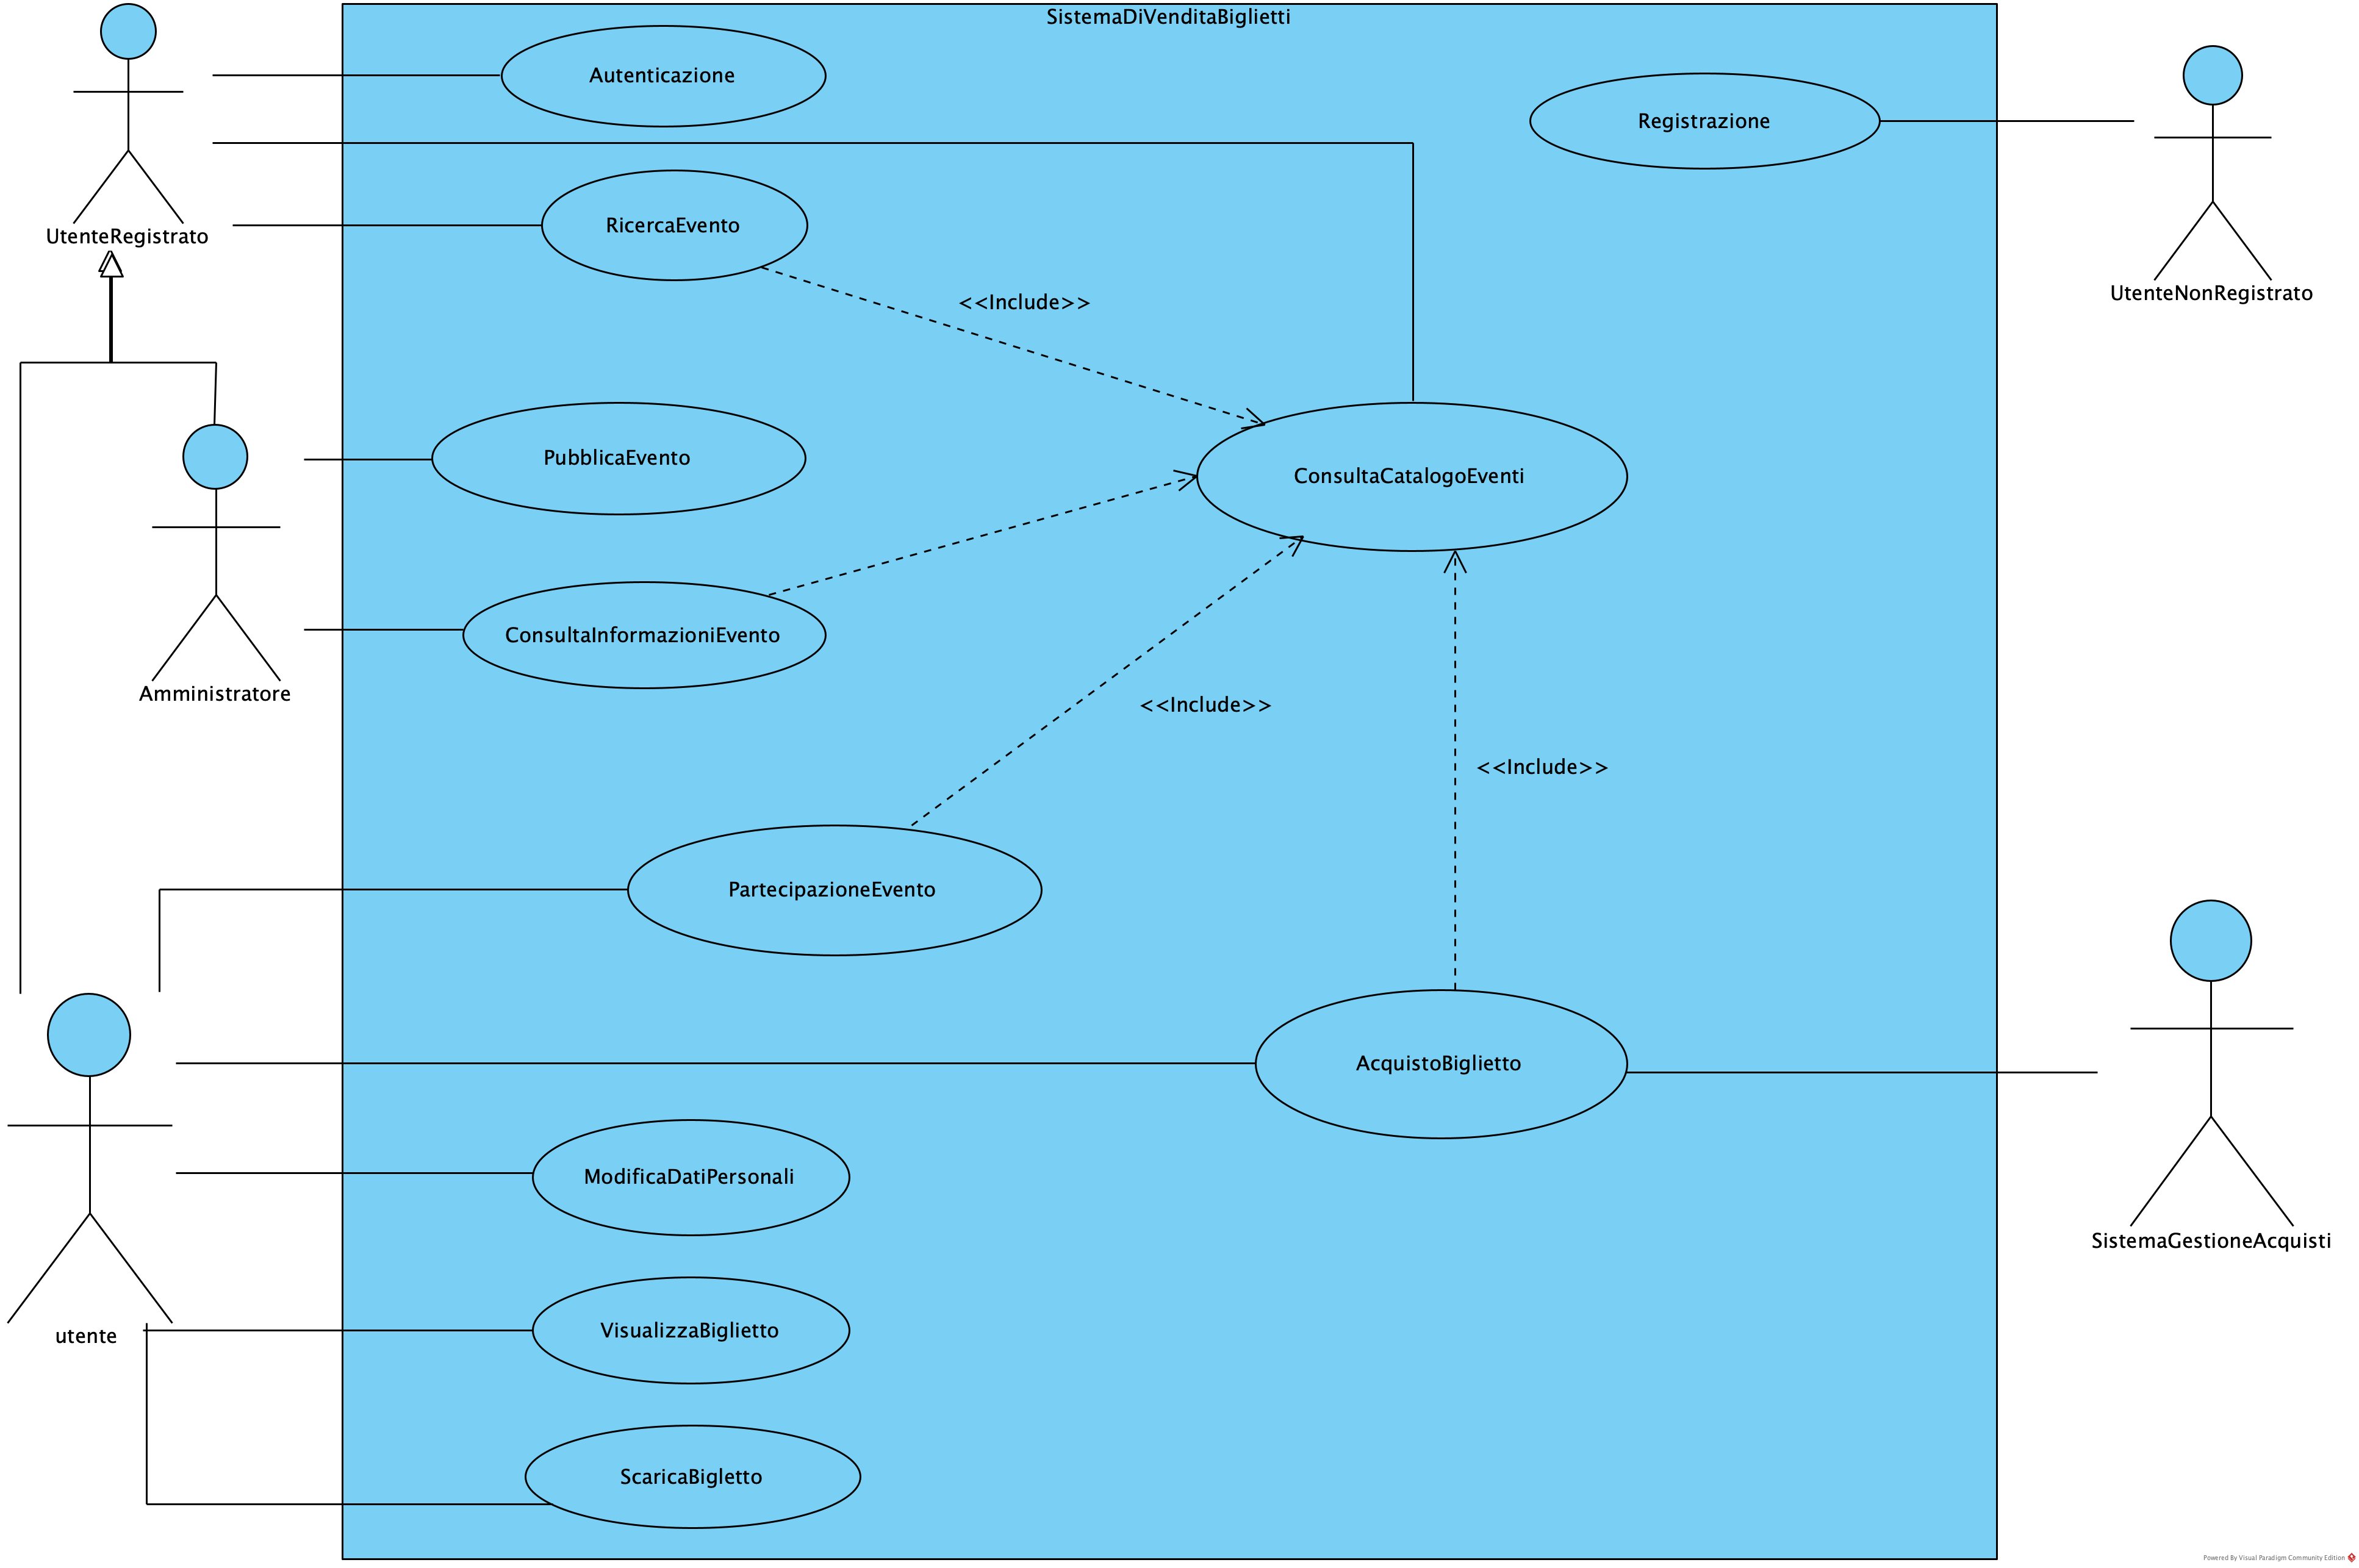
\includegraphics[width=\linewidth]{assets/casid'uso/usd.png}
\end{center}	

\clearpage
\section{Scenari}
\IncludeTable{capitoli/scenari/Registrazione}
\IncludeTable{capitoli/scenari/Autenticazione}
%\IncludeTable{capitoli/scenari/ModificaDatiPersonali}
\IncludeTable{capitoli/scenari/RichiediCatalogoEventi}
%\IncludeTable{capitoli/scenari/RicercaEvento}
%\IncludeTable{capitoli/scenari/VisualizzaBiglietto}
%\IncludeTable{capitoli/scenari/ConsultaStoricoBiglietti}
%\IncludeTable{capitoli/scenari/ScaricaBiglietto}
\IncludeTable{capitoli/scenari/AcquistaBiglietto}
\IncludeTable{capitoli/scenari/PubblicaEvento}
\IncludeTable{capitoli/scenari/PartecipazioneEvento}
\IncludeTable{capitoli/scenari/ConsultaEventiPubblicati}

\section{Diagramma delle Classi}
Di seguito riportiamo il diagramma delle classi di analisi.
\begin{figure}[H]
	\centering
	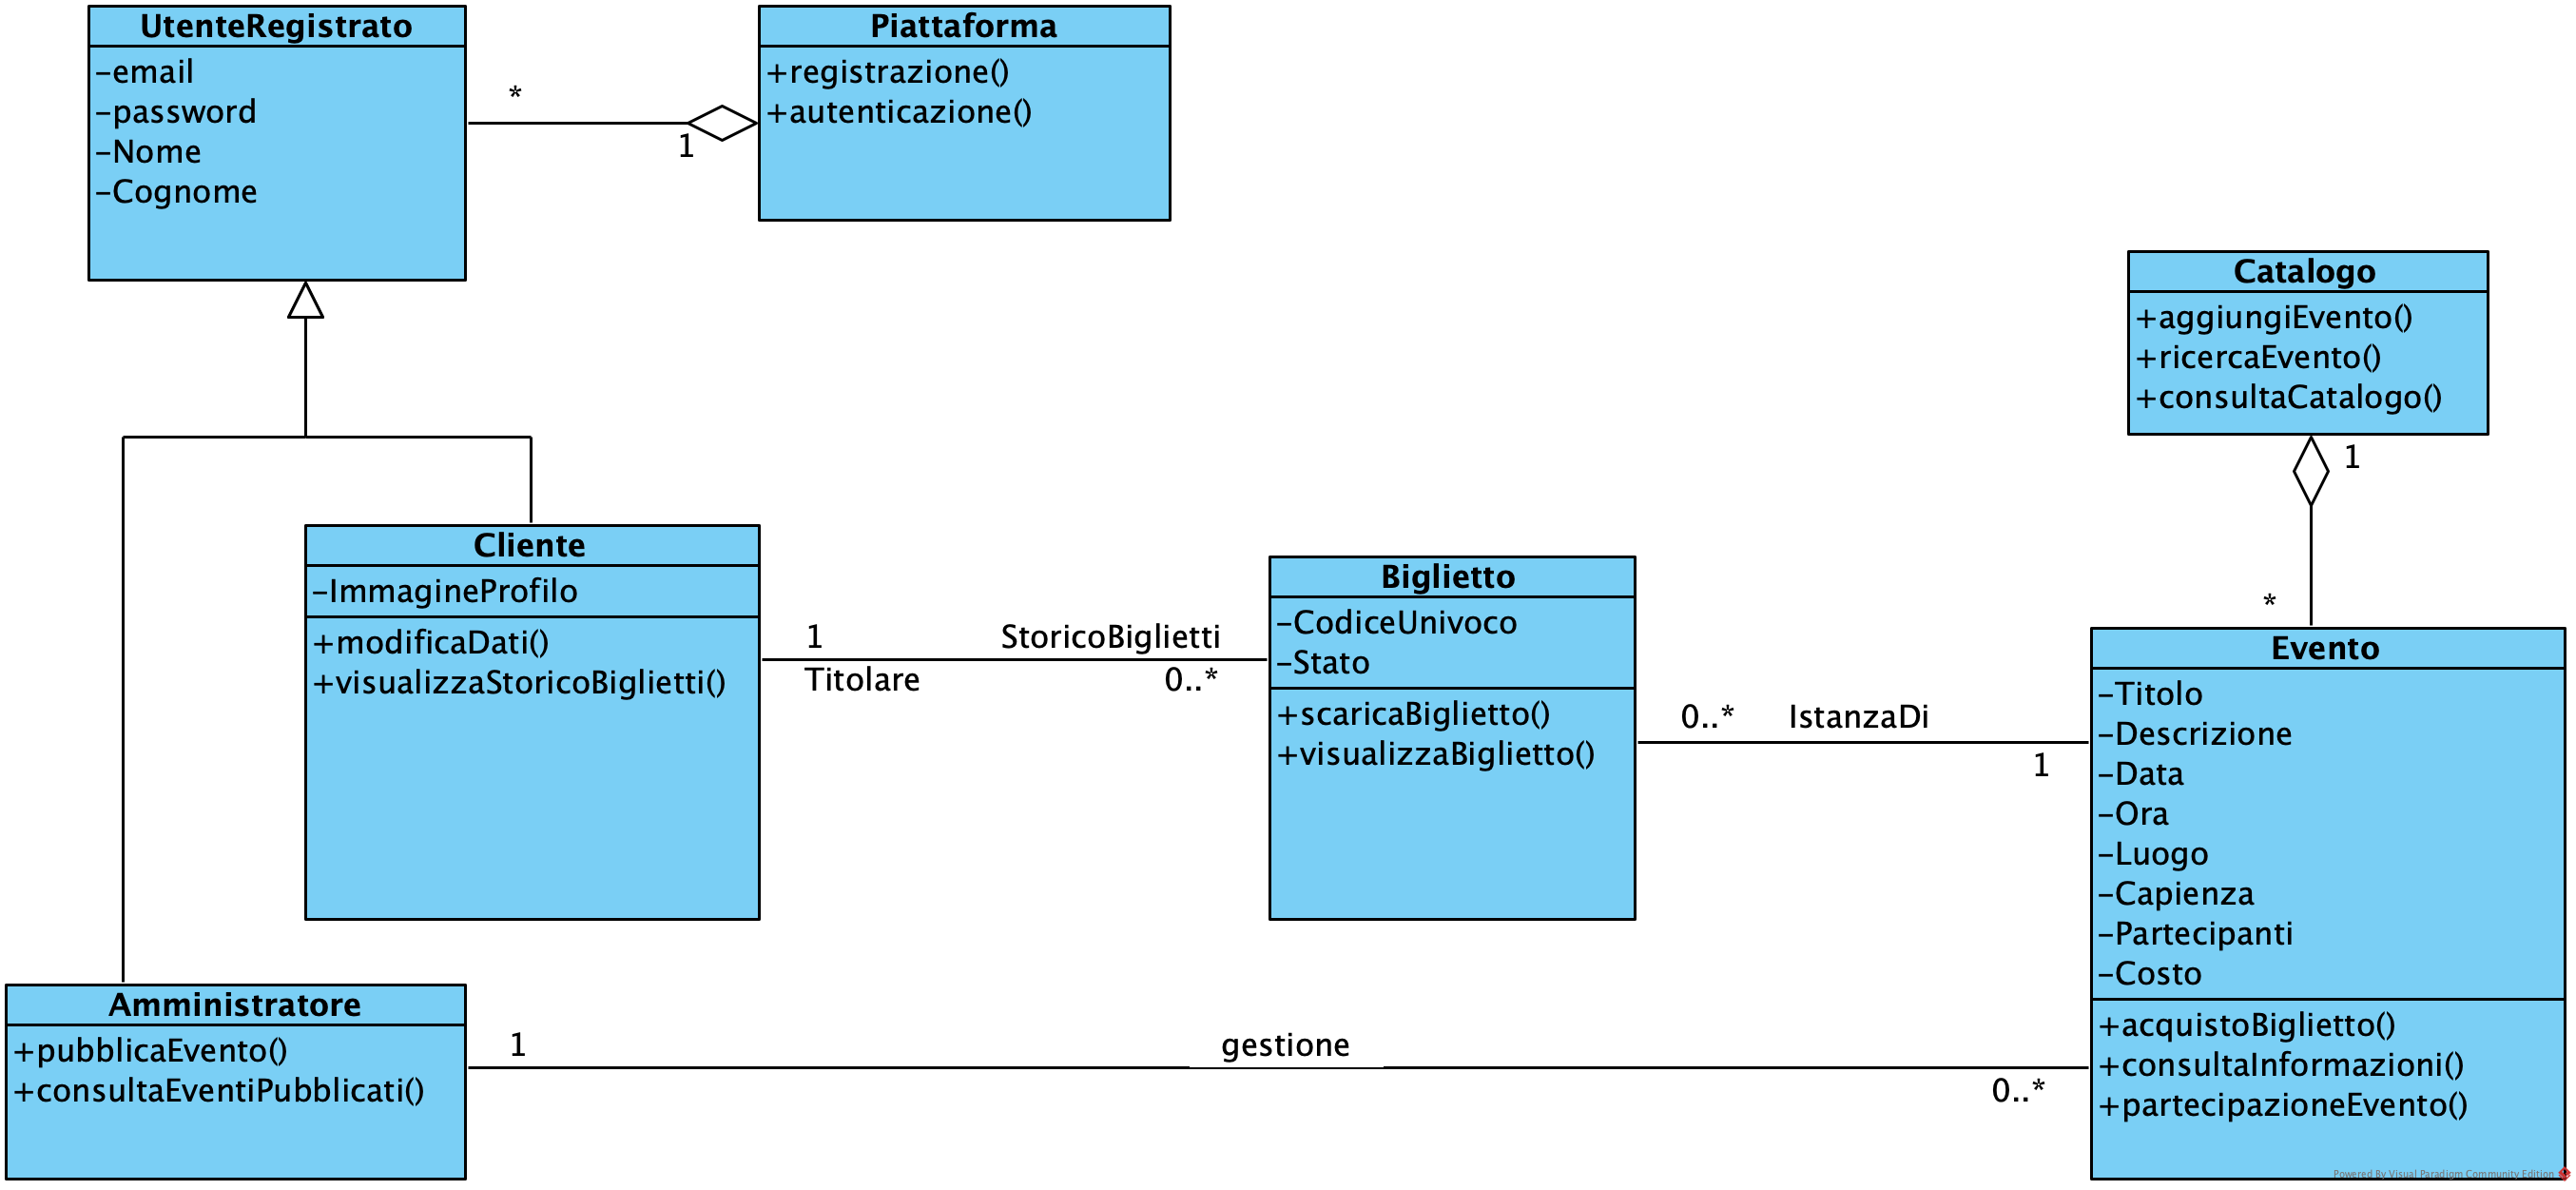
\includegraphics[width=0.8\linewidth]{assets/casid'uso/DiagrammaDelleClassi.png}
	\caption{Diagramma delle classi di analisi}
\end{figure}


\begin{table}[H]
	\centering
	\begin{tblr}{
	  colspec = {X[0.6,c] X[0.6,c]},
	  width = 1\linewidth, 
	  hlines, vlines,
	  row{1} = {bg=gray!30, font=\bfseries}
	}
	RESPONSABILITÀ & CLASSE \\
	Registrazione & SistemaGestioneEventi \\
	Autenticazione & SistemaGestioneEventi \\
	ModificaDati & Cliente \\
	VisualizzaStoricoBiglietti & Cliente \\
	CreazioneEvento & Amministratore \\
	ConsultaEventiPubblicati & Amministratore\\
	ScaricaBiglietto & Biglietto \\
	VisualizzaBiglietto & Biglietto \\
	AcquistoBiglietto & Evento \\
	PartecipazioneEvento & Evento \\
	ConsultaInformazioni & Evento \\
	AggiungiEvento & Catalogo \\
	RicercaEvento & Catalogo \\
	ConsultaCatalogo & Catalogo \\

	\end{tblr}
\end{table}


\begin{itemize}
    \item \textbf{Registrazione e Autenticazione:} \\
    Responsabilità del \textbf{SistemaGestioneEventi}, in quanto \emph{Information Expert} per la gestione degli oggetti \texttt{UtenteRegistrato}.
    
    \item \textbf{ModificaDati e VisualizzaStoricoBiglietti:} \\
    Responsabilità del \textbf{Cliente}, poiché operano direttamente sui suoi attributi e sulle entità a lui associate.
    
    \item \textbf{AcquistoBiglietto:} \\
    Assegnata alla classe \textbf{Evento}, in quanto \emph{Creator} degli oggetti \texttt{Biglietto}.
    
    \item \textbf{PartecipazioneEvento:} \\
    Gestita dalla classe \textbf{Evento}, seguendo il principio di \emph{Low Coupling} per minimizzare le dipendenze tra classi.
    
    \item \textbf{RicercaEvento, AggiungiEvento e ConsultaCatalogo:} \\
    Responsabilità della classe \textbf{Catalogo}, in quanto \emph{Information Expert} sugli oggetti \texttt{Evento} presenti nel sistema.
    
    \item \textbf{CreazioneEvento:} \\
    Di competenza dell'\textbf{Amministratore}, in quanto \emph{Creator} degli oggetti \texttt{Evento}.
    
    \item \textbf{ConsultaEventiPubblicati:} \\
    Assegnata all'\textbf{Amministratore}, poiché \emph{Information Expert} degli eventi da lui gestiti e pubblicati.
\end{itemize}

\newpage

\section{Diagrammi di sequenza}
\subsection{Registrazione}

La creazione del seguente diagramma di sequenza,ha fatto emergere la necessità di definire un metodo per la classe \textbf{Piattaforma}:
\texttt{controlloEmail(Email)},tale metodo consente alla \textbf{Piattaforma} di verificare che l'indirizzo email non sia già registrato nel sistema
\begin{figure}[H]
    \centering
    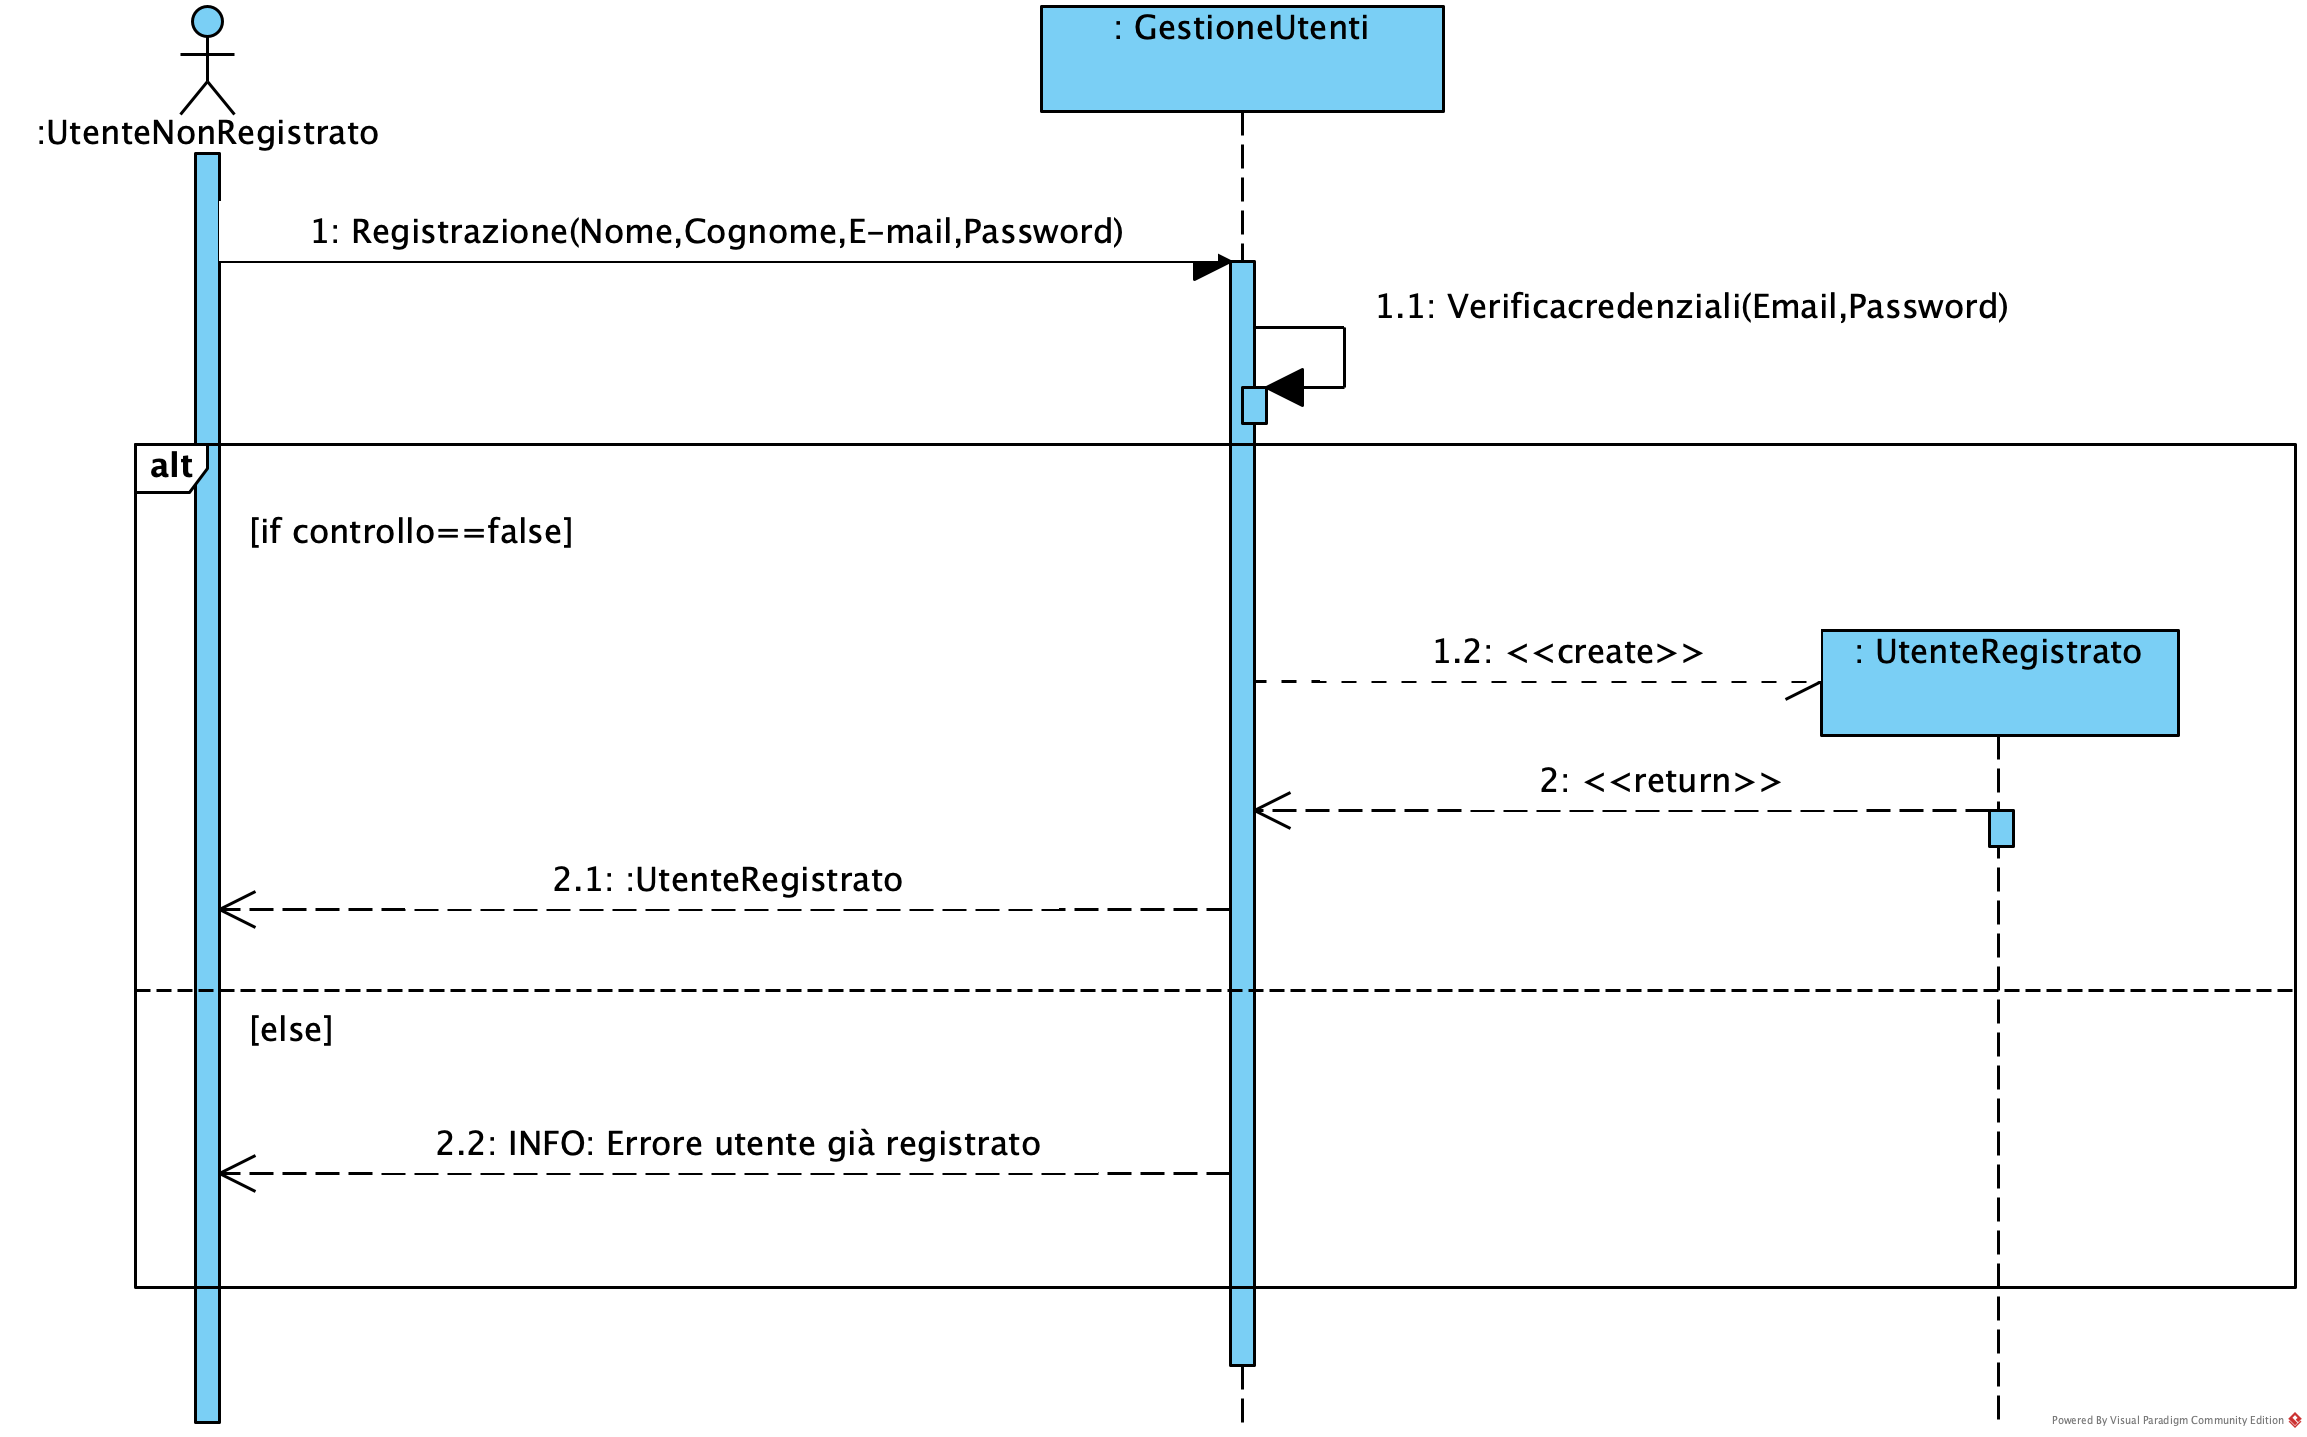
\includegraphics[width=0.8\linewidth]{assets/casid'uso/Registrazione.png}
    \caption{Diagramma di sequenza per il caso d'uso \emph{Registrazione}}
    \label{fig:registrazione}
\end{figure}

\subsection{Autenticazione}
Il diagramma di sequenza ha evidenziato la necessità del metodo \texttt{controlloCredenziali(email, password)} per la classe \textbf{Piattafroma}, che permette di verificare le credenziali di accesso.
\begin{figure}[H]
    \hspace{4cm}
    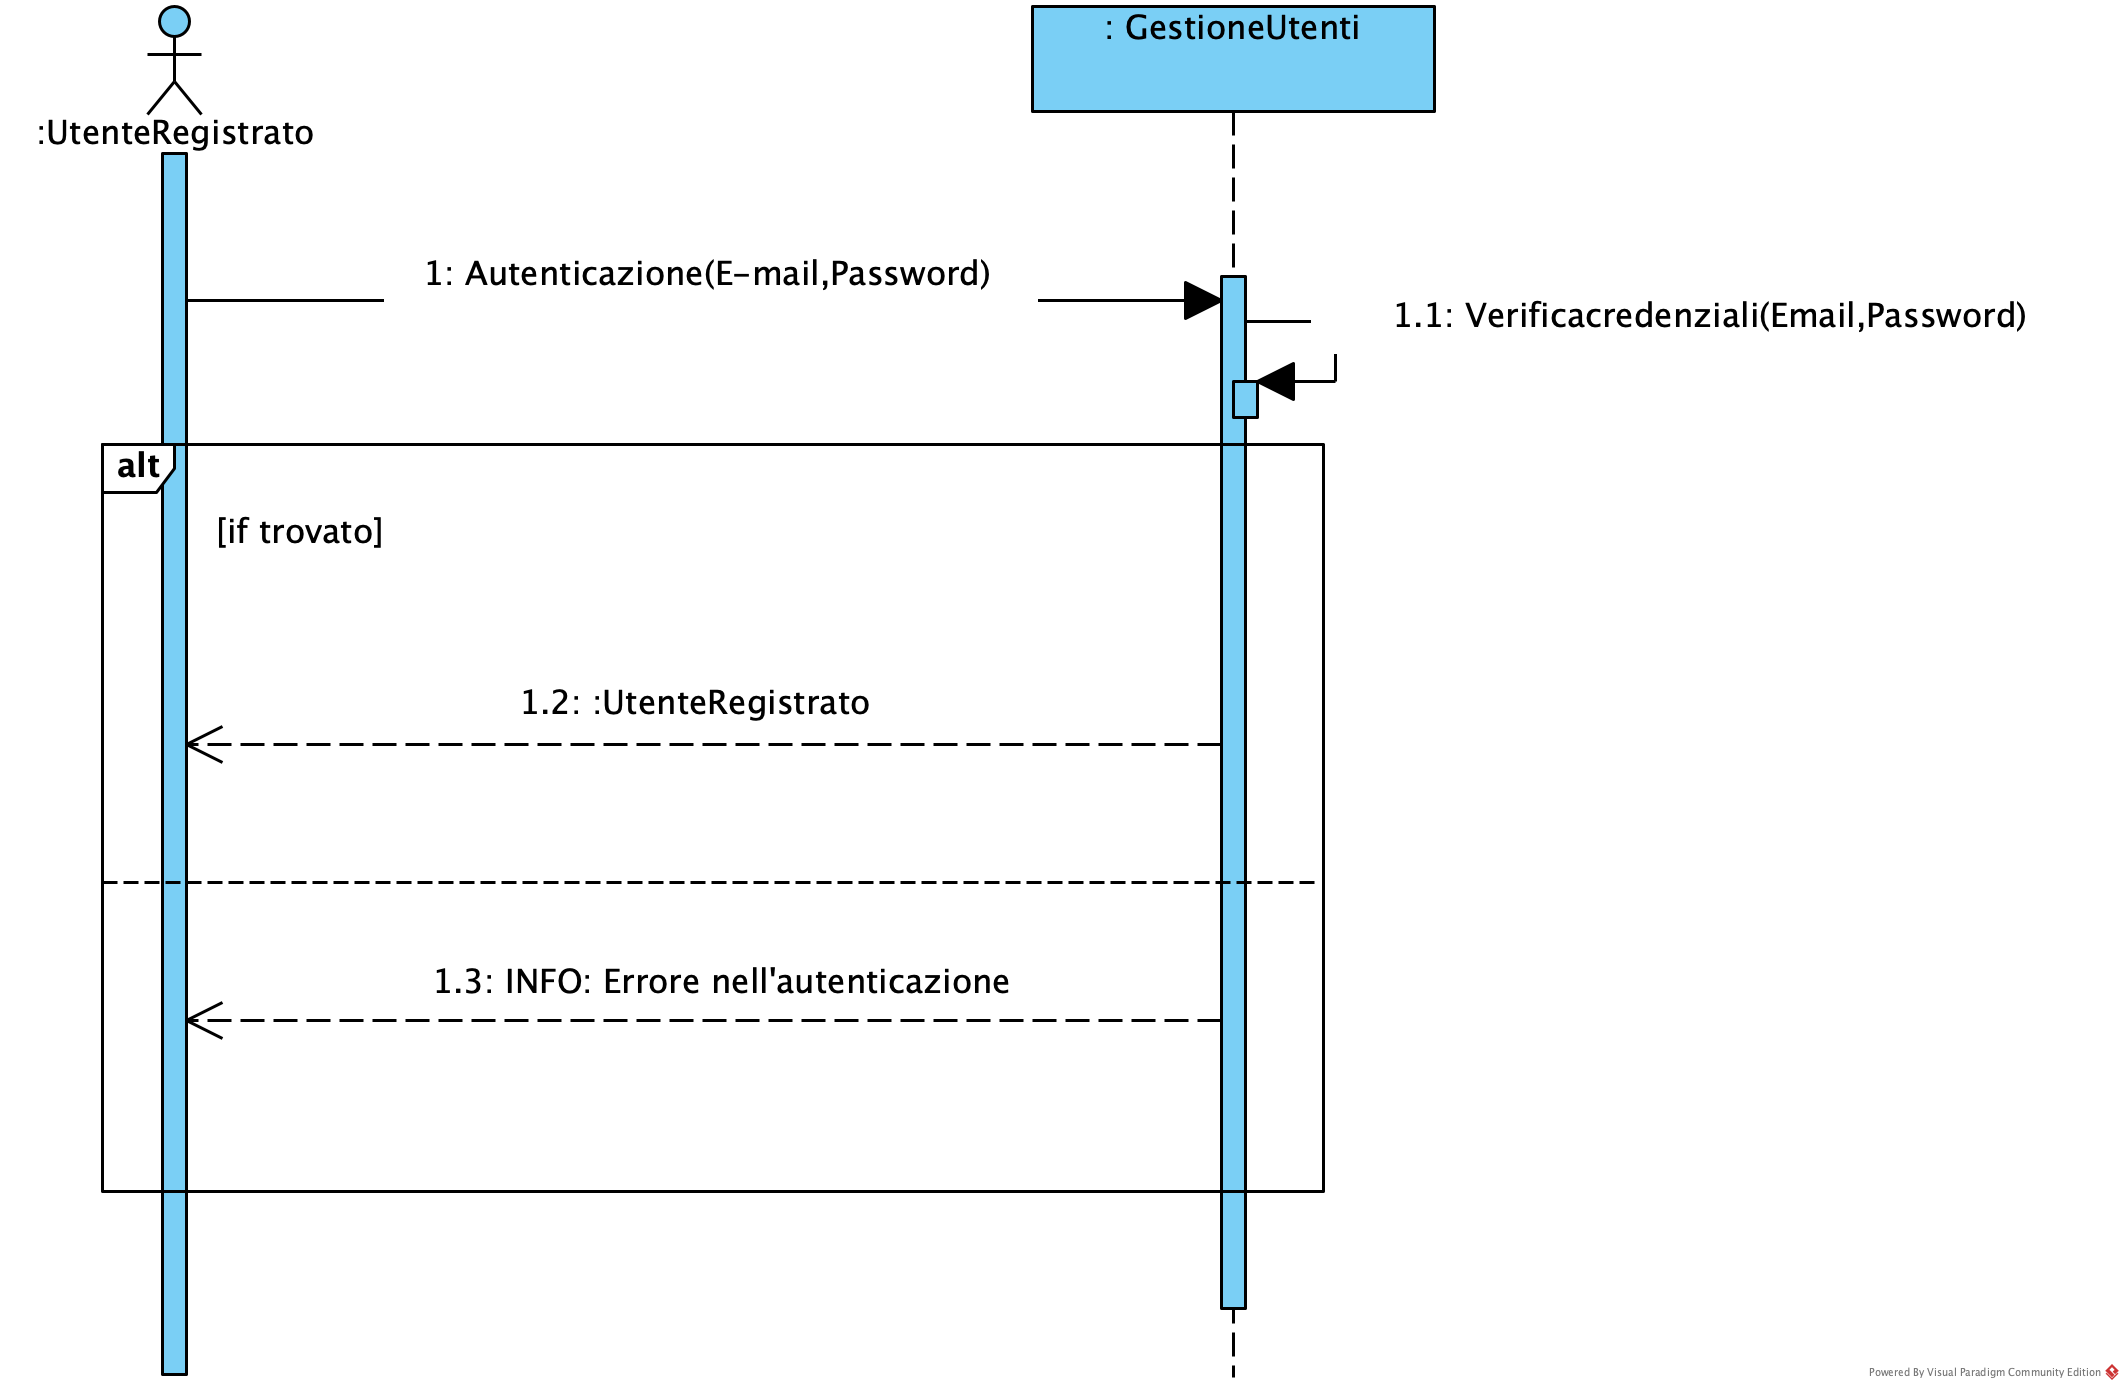
\includegraphics[width=0.8\linewidth]{assets/casid'uso/Autenticazione.png}
    \caption{Diagramma di sequenza per il caso d'uso \emph{Autenticazione}}
    \label{fig:autenticazione}
\end{figure}

\subsection{PubblicaEvento}

Il diagramma di sequenza ha evidenziato la necessità del metodo \texttt{verificaValidità(Titolo,Data)} per la classe \textbf{Amministratore}, che permette di verificare che non esite nel sistema un evento con lo stesso titolo e che la data sia maggiore di quella della pubblicazione

\begin{figure}[H]
    \centering
    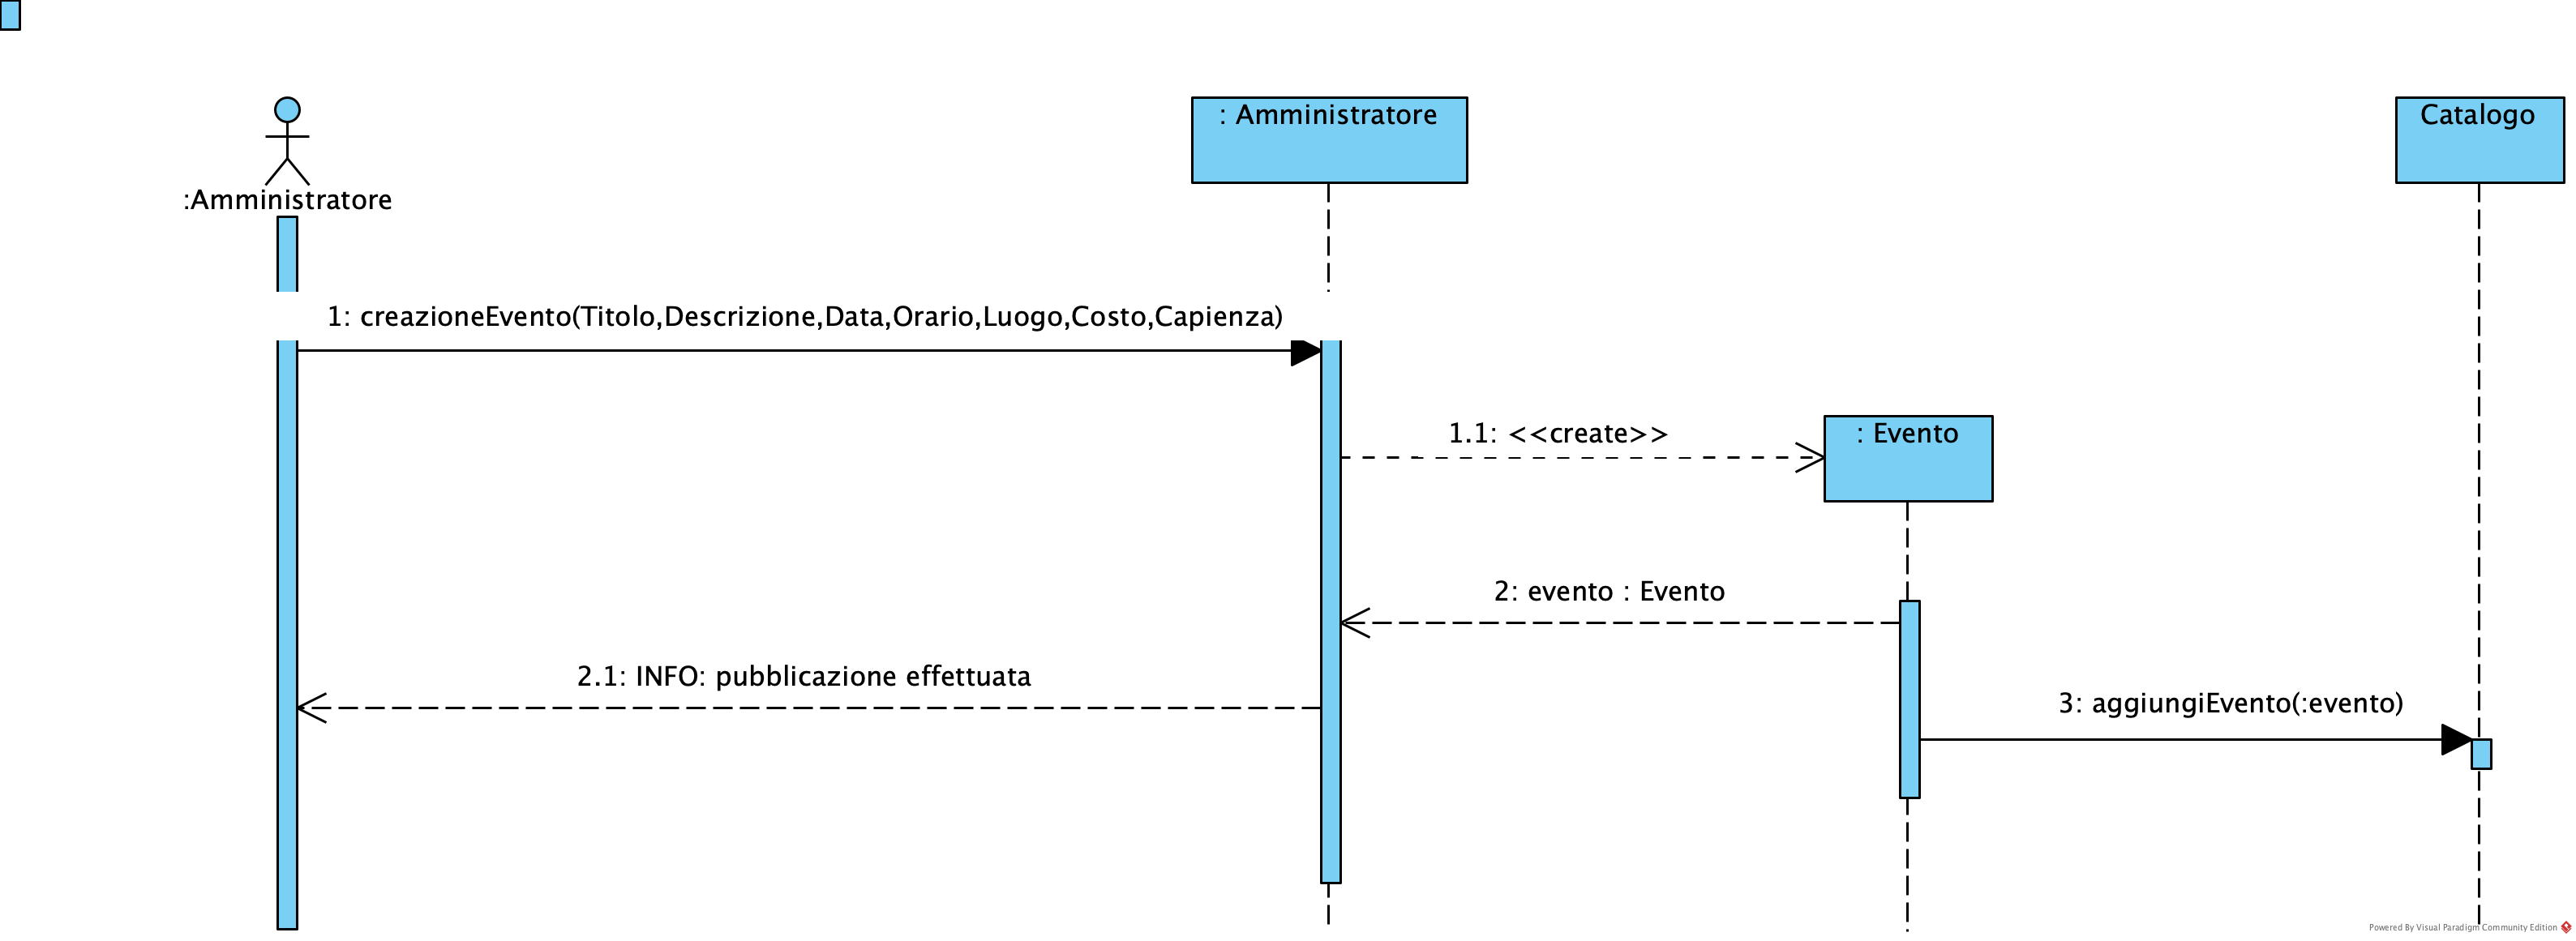
\includegraphics[width=\linewidth]{assets/casid'uso/PubblicaEvento.png}
    \caption{Diagramma di sequenza per il caso d'uso \emph{PubblicaEvento}}
    \label{fig:pubblicaevento}
\end{figure}

\subsection{ConsultaEventiPubblicati}

\begin{center}
    Il diagramma di sequenza del caso d'uso \textit{ConsultaEventiPubblicati} mostra la necessità di una responsabilità \textbf{getListaPartecipanti()} da parte dell'evento

    \vspace{2ex}
    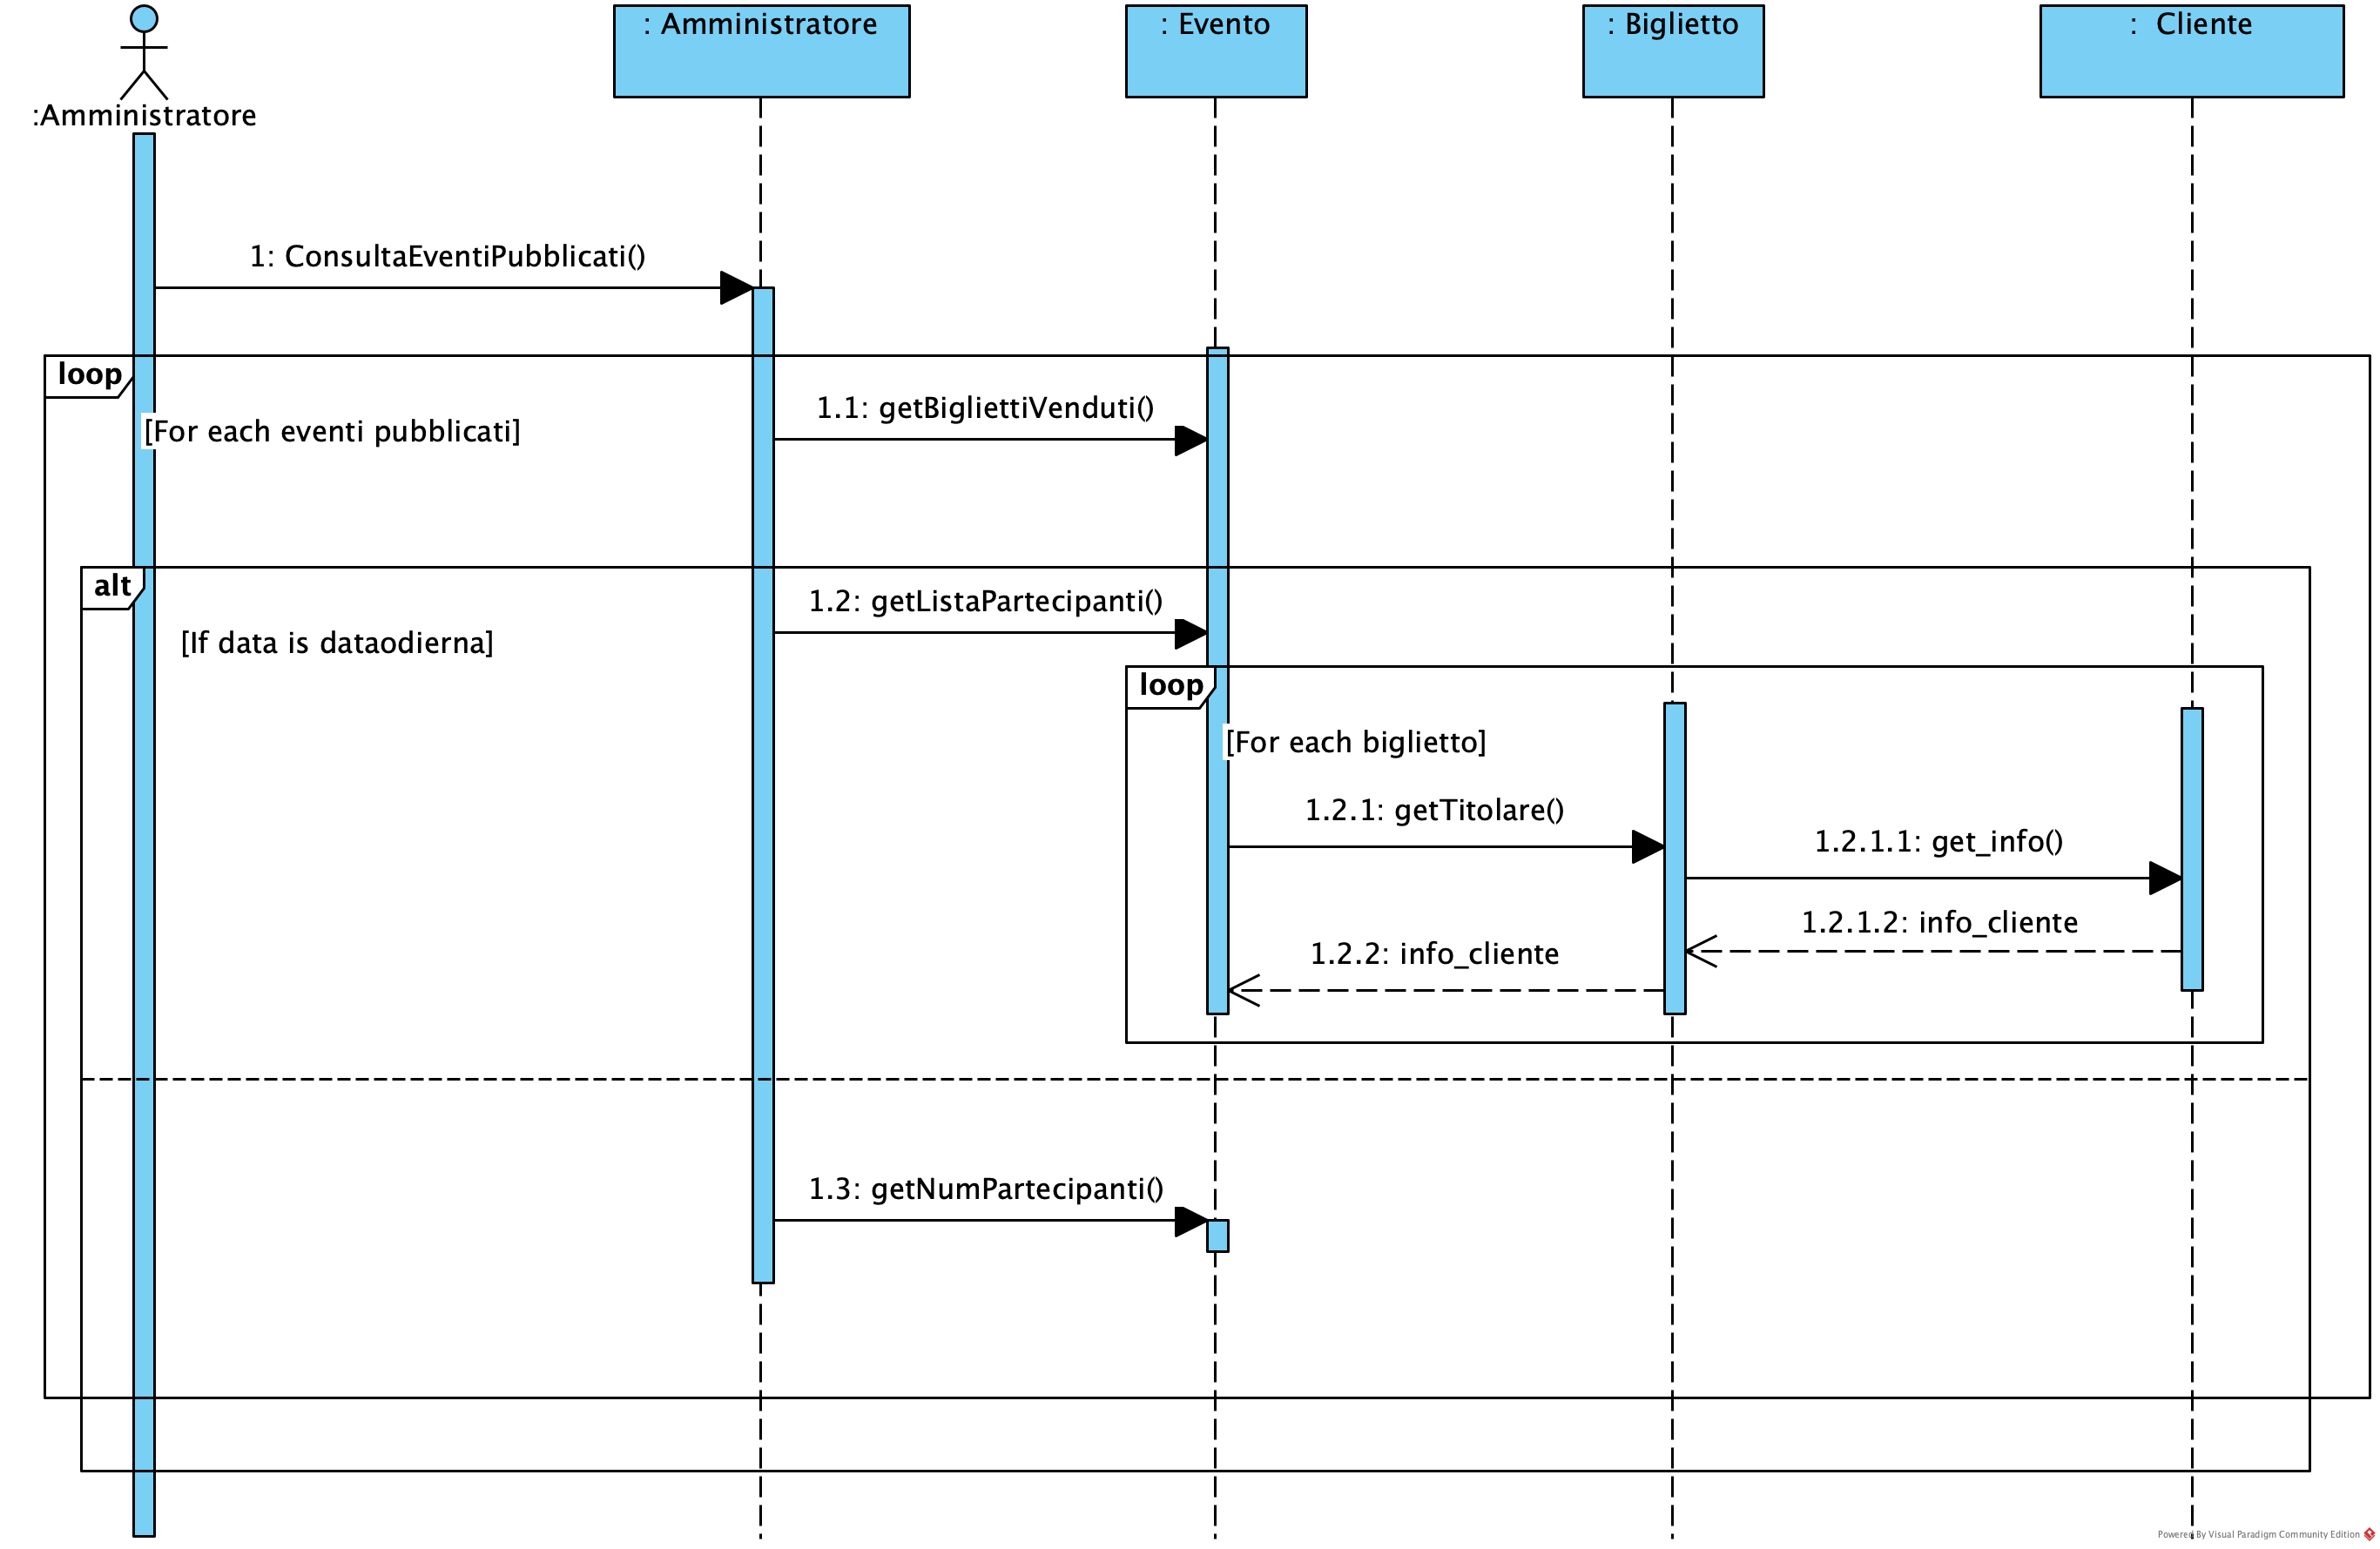
\includegraphics[width=0.8\linewidth]{assets/casid'uso/ConsultaEventiPubblicati.png}

    \vspace{1ex}
    \textbf{Figura:} Diagramma di sequenza per il caso d’uso \textit{ConsultaEventiPubblicati}
\end{center}

\subsection{AcquistoBiglietti}

Il diagramma di sequenza ha evidenziato diverse responsabilità: per la classe \textbf{Evento} i metodi \texttt{verificaDisponibilità()}, \texttt{creazioneIdUnivoco()} e \texttt{InviaDatiPagamento(NomeTitolare, CognomeTitolare,informazioniCarta,DataScadenza)}, mentre per la classe \textbf{Cliente} il metodo \texttt{haBigliettoPerEvento(evento)} per verificare eventuali acquisti precedenti.

\begin{figure}[H]
    \centering
    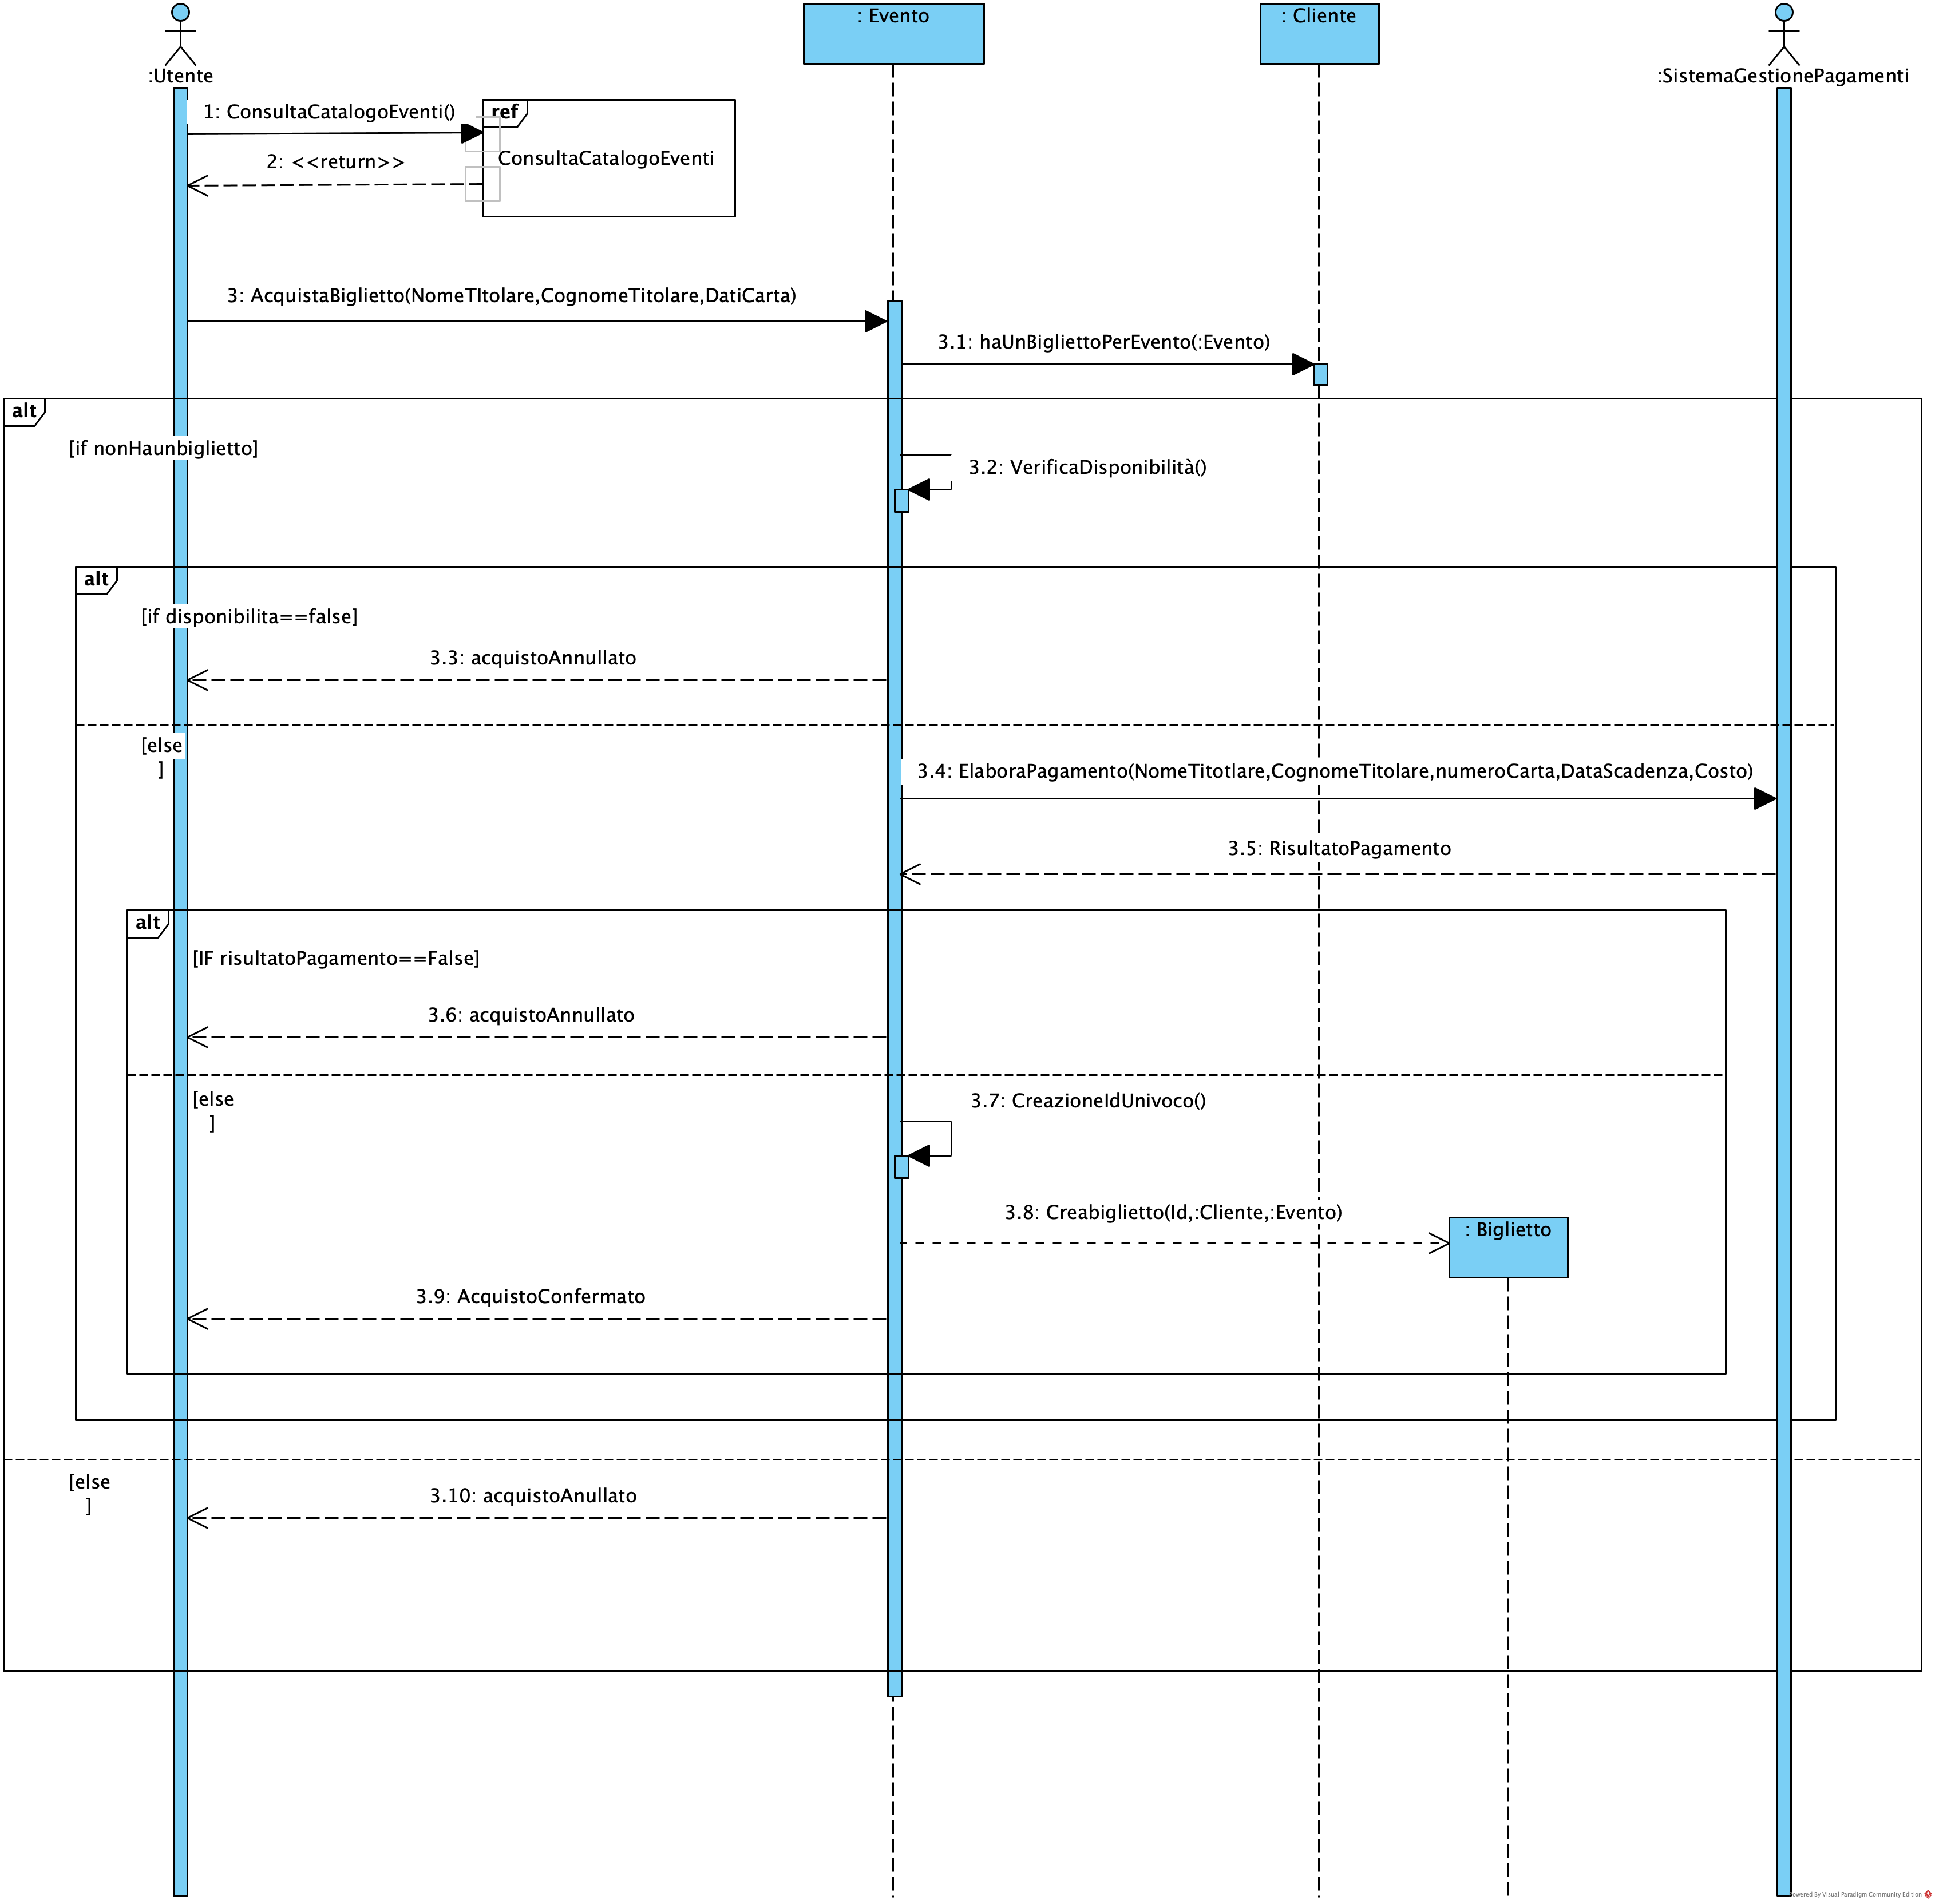
\includegraphics[width=0.8\linewidth]{assets/casid'uso/AcquistoBiglietto.png}
    \caption{Diagramma di sequenza per il caso d'uso \emph{AcquistoBiglietto}}
    \label{fig:acquistobiglietto}
\end{figure}



\subsection{PartecipazioneEvento}

Il diagramma di sequenza ha evidenziato la necessità di aggiungere il metodo \texttt{verificaCodice()} per la classe \textbf{Evento} e il metodo \texttt{validaBiglietto()} per la classe \textbf{Biglietto}, necessari per gestire la partecipazione degli utenti agli eventi.

\begin{figure}[H]
    \centering
    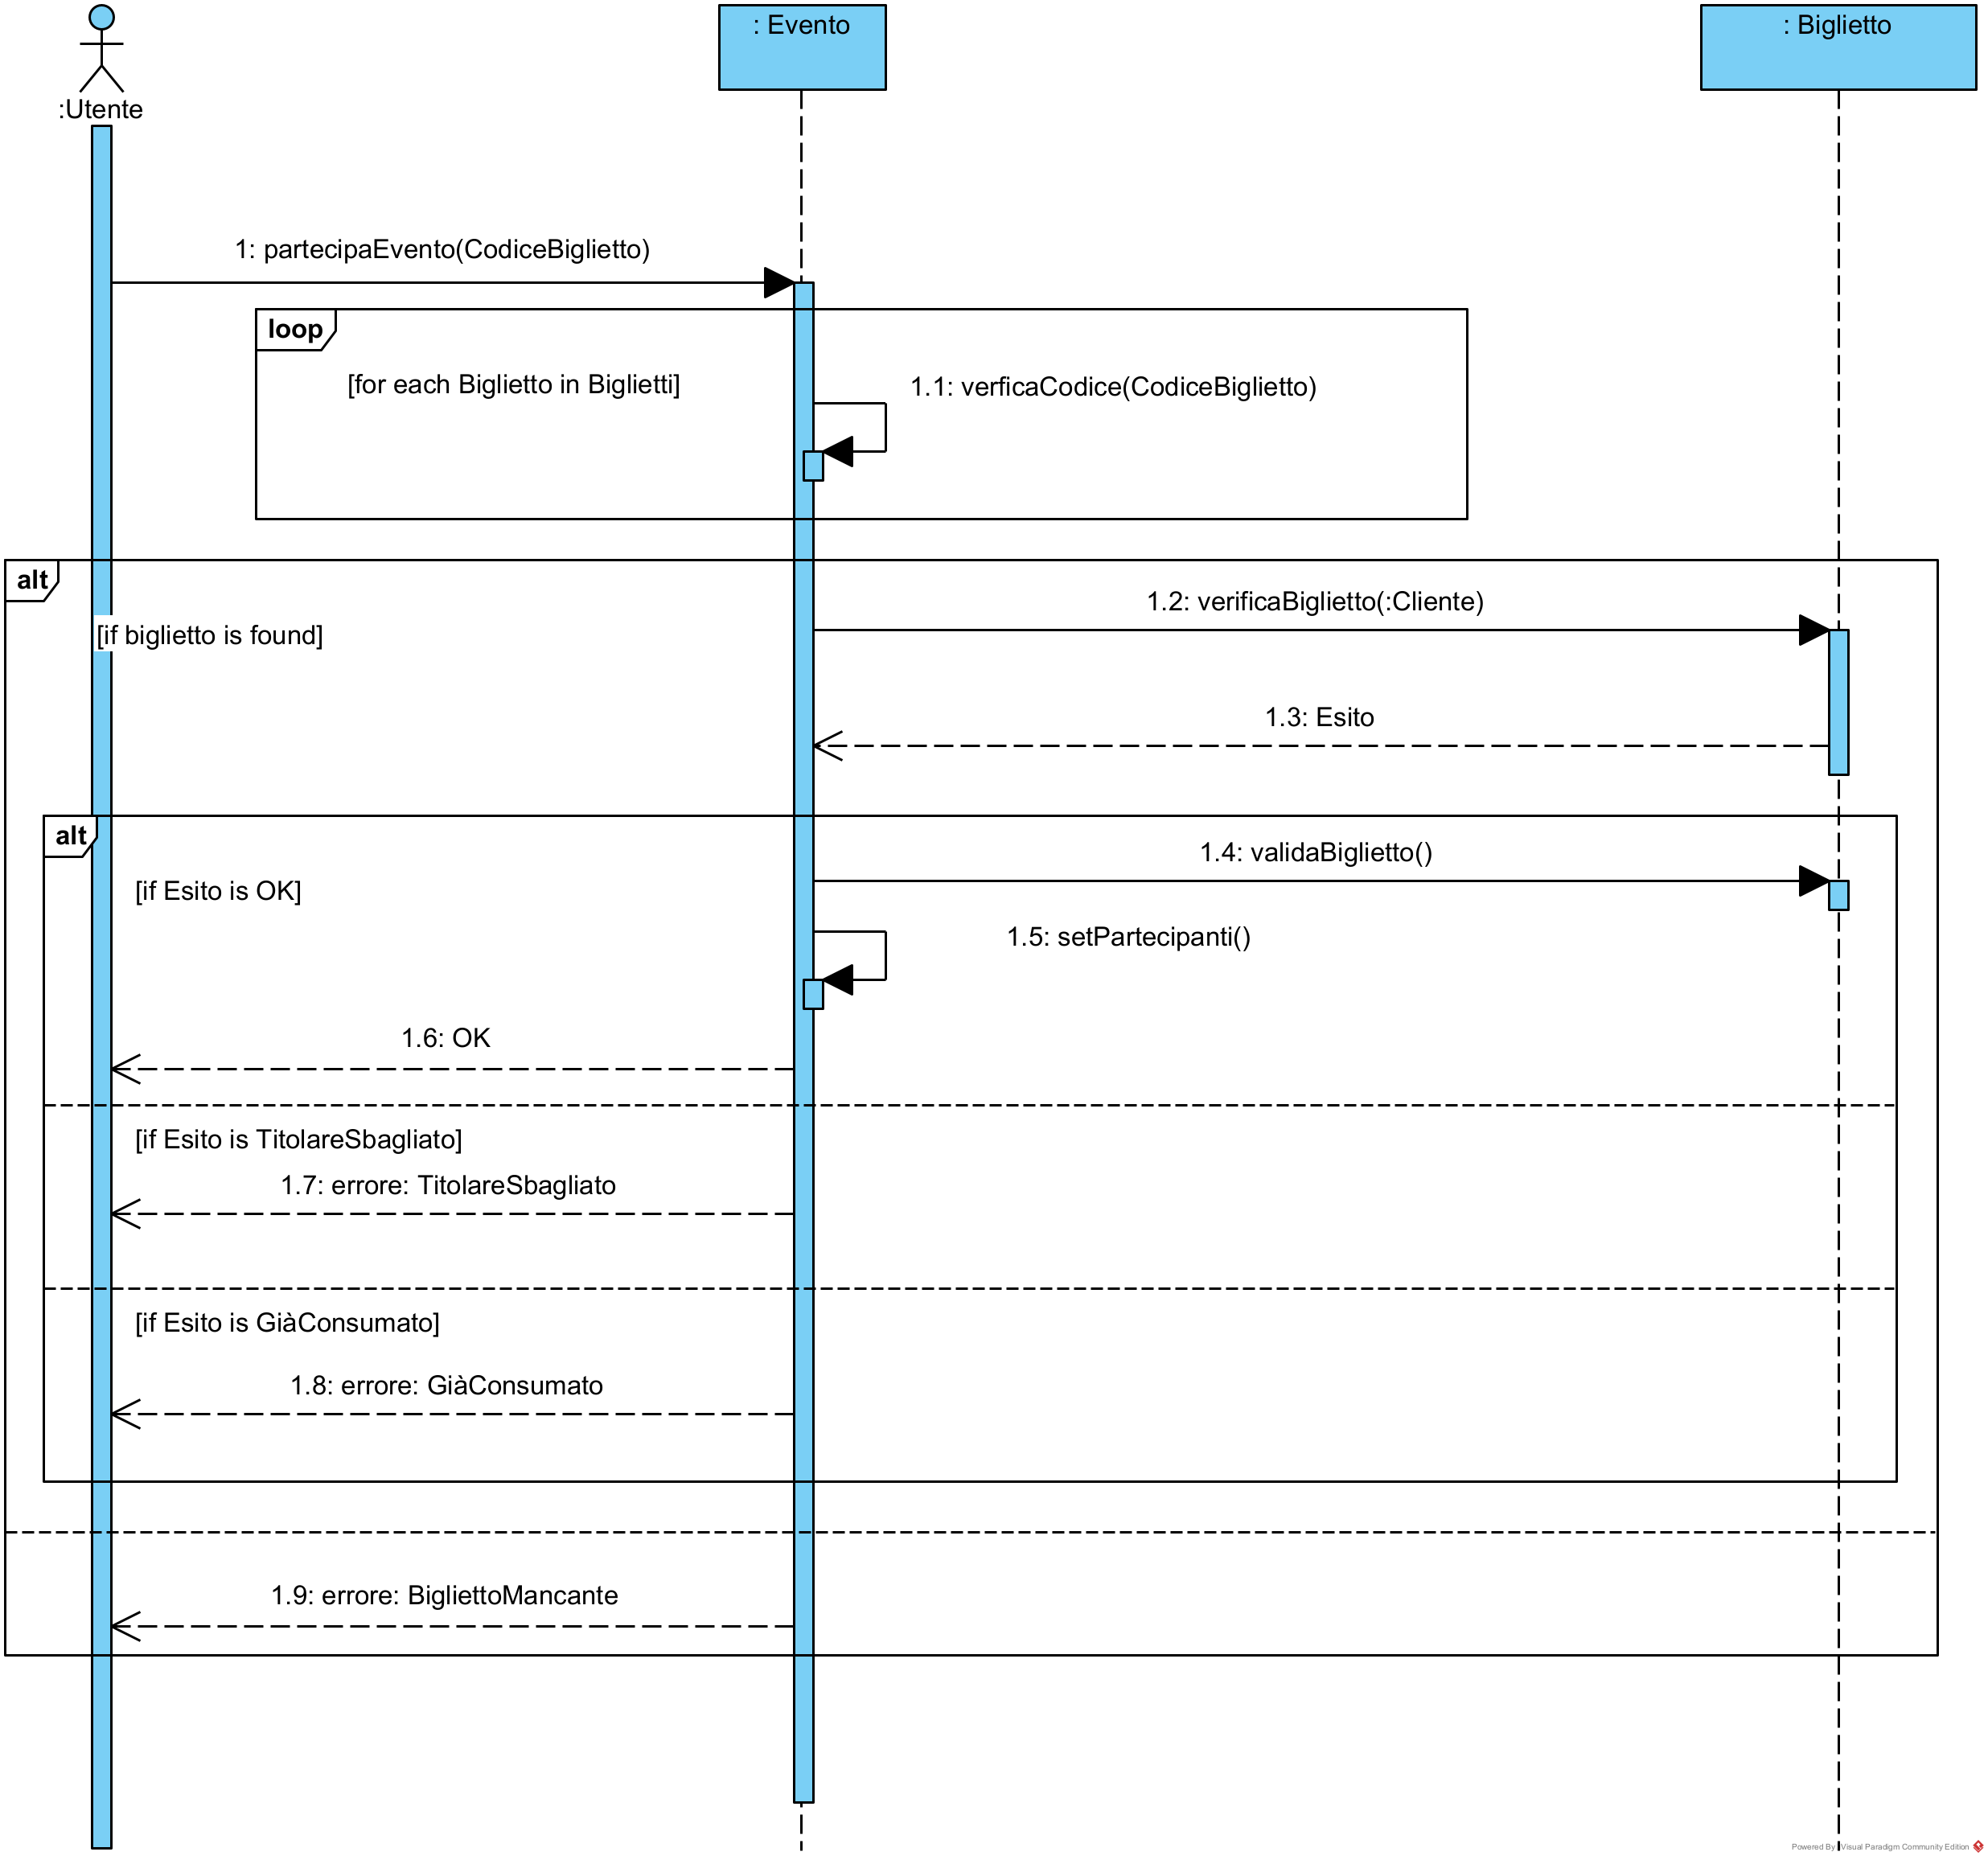
\includegraphics[height=0.38\textheight]{assets/casid'uso/PartecipazioneEvento.png}
    \caption{Diagramma di sequenza per il caso d'uso \emph{PartecipazioneEvento}}
    \label{fig:partecipazione}
\end{figure}

\section{Diagramma delle classi raffinato}
\begin{center}	
	\vspace{1ex}
	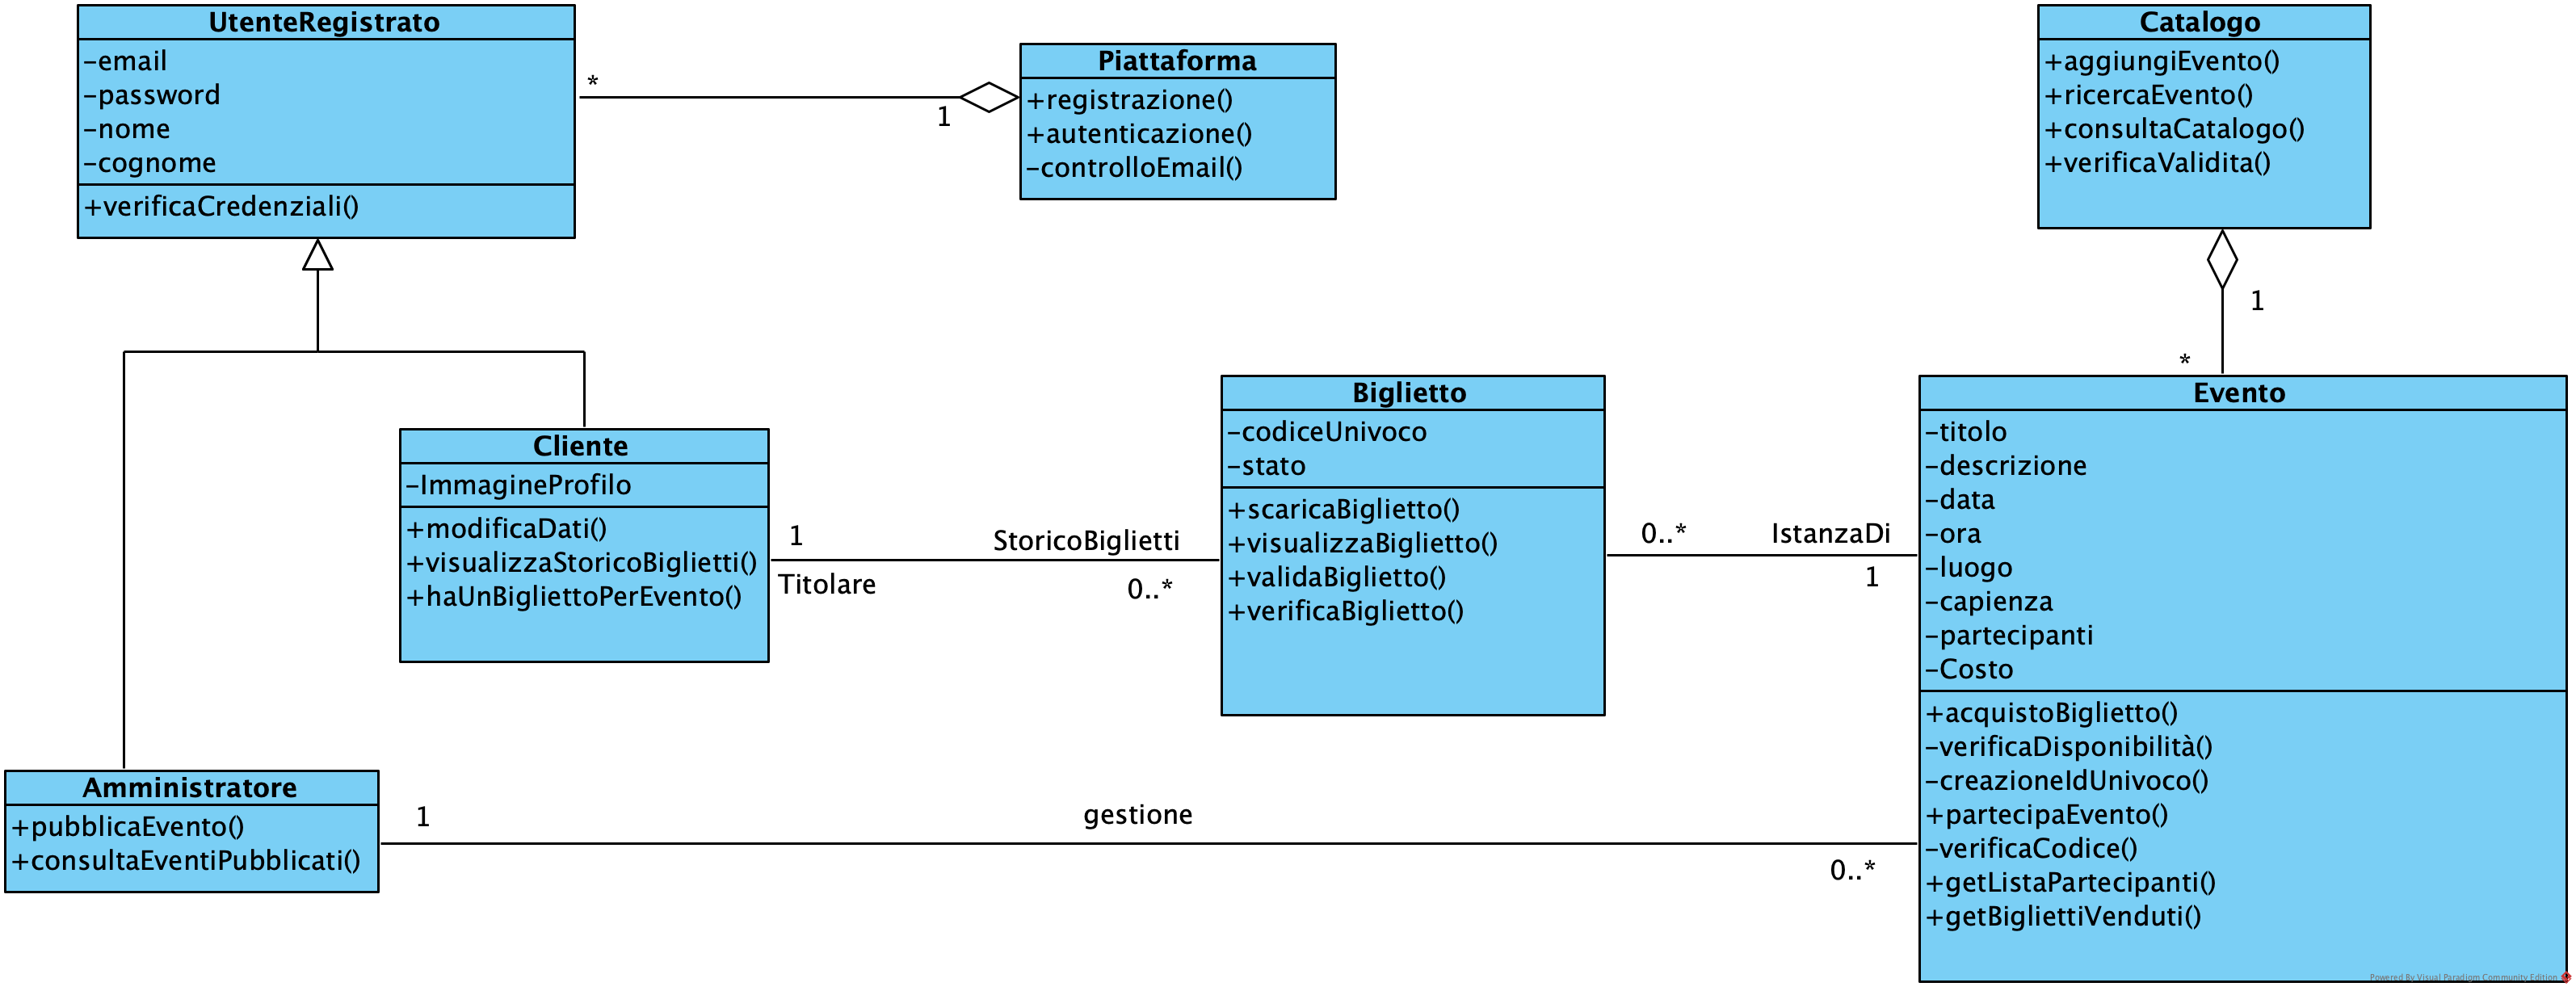
\includegraphics[height=0.38\linewidth]{assets/casid'uso/DiagrammaDelleClassiRaffinato.png}
	\vspace{1ex}
\end{center}




\end{document}